\documentclass[12pt]{article}

% ----------------------------------------------------------------------
% Define external packages, language, margins, fonts, new commands 
% and colors
% ----------------------------------------------------------------------
\usepackage[utf8]{inputenc} % Codification
\usepackage[english]{babel} % Writing idiom

\usepackage{listings}
\usepackage[dvipsnames]{xcolor}
\usepackage[most]{tcolorbox}
\usepackage{float}

\definecolor{codebg}{RGB}{245,245,245}
\definecolor{codeframe}{RGB}{200,200,200}

\lstdefinestyle{CiscoStyle}{
    backgroundcolor=\color{codebg},
    basicstyle=\ttfamily\small,
    keywordstyle=\color{blue},
    commentstyle=\color{gray},
    breaklines=true,
    showstringspaces=false,
    columns=fullflexible
}

\newtcblisting{configbox}{
    listing only,
    colback=codebg,
    colframe=codeframe,
    arc=3mm,
    boxrule=0.5pt,
    left=2mm,
    right=2mm,
    top=1mm,
    bottom=1mm,
    listing options={style=CiscoStyle}
}

\newtcblisting{largeconfigbox}{
    listing only,
    breakable,
    colback=codebg,
    colframe=codeframe,
    arc=3mm,
    boxrule=0.5pt,
    listing options={
        style=CiscoStyle,
        basicstyle=\ttfamily\scriptsize
    }
}

\usepackage{graphicx}
\usepackage[export]{adjustbox} % Align images
\usepackage{amsmath} % Extra commands for math mode
\usepackage{amssymb} % Mathematical symbols
\usepackage{anysize} % Personalize margins
    \marginsize{2cm}{2cm}{2cm}{2cm} % {left}{right}{above}{below}
\usepackage{appendix} % Appendices
\usepackage{cancel} % Expression cancellation
\usepackage{caption} % Captions
    \captionsetup{labelfont={bf}}
\usepackage{cite} % Citations, like [1 - 3]
\usepackage{color} % Text coloring
\usepackage{fancyhdr} % Head note and footnote
    \pagestyle{fancy}
    \fancyhf{}
    \fancyhead[L]{\footnotesize IST} % Left of Head note
    \fancyhead[R]{\footnotesize ULisboa} % Right of Head note
    \fancyfoot[L]{\footnotesize SAAR} % Left of Footnote
    \fancyfoot[C]{\thepage} % Center of Footnote
    \fancyfoot[R]{\footnotesize METI} % Right of Footnote
    \renewcommand{\footrulewidth}{0.4pt} % Footnote rule
\usepackage{float} % Utilization of [H] in figures
\usepackage{graphicx} % Figures in LaTeX
\usepackage[colorlinks = true, plainpages = true, linkcolor = istblue, urlcolor = istblue, citecolor = istblue, anchorcolor = istblue]{hyperref}
\usepackage{indentfirst} % First paragraph
\usepackage[super]{nth} % Superscripts
\usepackage{siunitx} % SI units
\usepackage{subcaption} % Subfigures
\usepackage{titlesec} % Font
    \titleformat{\section}{\Large\bfseries}{\thesection}{1em}{}
    \titleformat{\subsection}{\large\bfseries}{\thesubsection}{1em}{}
    \titleformat{\subsubsection}{\normalsize\bfseries}{\thesubsubsection}{1em}{}
    \fancyfoot[C]{\thepage}

% Random text (not needed)
\usepackage{lipsum}
\usepackage{duckuments}

% New and re-newcommands
\newcommand{\sen}{\operatorname{\sen}} % Sine function definition
\newcommand{\HRule}{\rule{\linewidth}{0.5mm}} % Specific rule definition
\renewcommand{\appendixpagename}{\LARGE Appendices}

% Colors
\definecolor{istblue}{RGB}{3, 171, 230}
\definecolor{dkgreen}{rgb}{0,0.6,0}
\definecolor{gray}{rgb}{0.5,0.5,0.5}

%%%%%%%%%%%%%%%%%%%%%%%%%%%%%%%%%%%%%%%%%%%%%%%%%%%%%%%%%%%%%%%%%%%%%%%%
%                                 Document                             %
%%%%%%%%%%%%%%%%%%%%%%%%%%%%%%%%%%%%%%%%%%%%%%%%%%%%%%%%%%%%%%%%%%%%%%%%
\begin{document}

% ----------------------------------------------------------------------
% Cover
% ----------------------------------------------------------------------
\begin{center}
    \begin{figure}
        \vspace{-1.0cm}
        
\includegraphics[scale = 0.25, left]{../Images/IST_A.png} % IST logo
    \end{figure}
    \mbox{}\\[2.0cm]
    \textsc{\Huge Advanced Network Security and Architectures}\\[2.5cm]
    \textsc{\LARGE METI}\\[2.0cm]
    \HRule\\[0.4cm]
    {\large \bf {Report Module 1} [\texttt{EN}]}\\[0.2cm]
    \HRule\\[1.5cm]
\end{center}

\begin{flushleft}
    \textbf{Authors:}
\end{flushleft}

\begin{center}
    \begin{minipage}{0.5\textwidth}
        \begin{flushleft}
            José Oliveira (103771)\\
            Afonso Mendes (116024)\\
            Tiago Videira (116069)
        \end{flushleft}
    \end{minipage}%
    \begin{minipage}{0.5\textwidth}
        \begin{flushright}
            \href{mailto:jose.novais.oliveira@tecnico.ulisboa.pt}{\texttt{jose.novais.oliveira@tecnico.ulisboa.pt}}\\
            \href{mailto:afonsofmendes@tecnico.ulisboa.pt}{\texttt{afonsofmendes@tecnico.ulisboa.pt}}\\
            \href{mailto:tiago.g.videira@tecnico.ulisboa.pt}{\texttt{tiago.g.videira@tecnico.ulisboa.pt}}
        \end{flushright}
    \end{minipage}
\end{center}
    
\begin{flushleft}
    \large $\boxed{\text{\bf Group 3 }}$\\[4.0cm]
\end{flushleft}
    
\begin{center}
    \large \bf 2025/2026 -- \nth{2} Semester, P4
\end{center}

\thispagestyle{empty}

\setcounter{page}{0}

\newpage

% ----------------------------------------------------------------------
% Contents
% ----------------------------------------------------------------------
\tableofcontents 

\newpage

% ----------------------------------------------------------------------
% Body
% ----------------------------------------------------------------------

\section{Introduction}

FAZER APENAS NO FIM DOS 3 LABS

\newpage

\section {Network attacks and countermeasures}

\subsection{Objective}

The main objective of this laboratory work is to study and experimentally evaluate a set of common network attacks and their corresponding countermeasures in a controlled environment using GNS3.

In particular, the following attacks are addressed:

\begin{itemize}
    \item \textbf{MAC table overflow:} to understand how a switch can be forced to behave as a hub by saturating its MAC address table, and to evaluate mitigation mechanisms such as port security.
    
    \item \textbf{DHCP spoofing:} to demonstrate how a rogue DHCP server can provide malicious network configurations to clients, and to analyze the effectiveness of DHCP snooping as a countermeasure.
    
    \item \textbf{ARP poisoning (Man-in-the-Middle):} to perform a MitM attack by manipulating ARP tables, and to study the use of Dynamic ARP Inspection (DAI) for protection.
    
    \item \textbf{DNS spoofing:} to analyze how a victim can be redirected to a fake web server through DNS manipulation combined with ARP poisoning.
    
    \item \textbf{RIP poisoning:} to investigate how routing tables can be corrupted using forged RIP messages, leading to traffic redirection, and to explore authentication-based defenses.
\end{itemize}

Additionally, this work aims to:

\begin{itemize}
    \item Analyze network behavior through packet captures using Wireshark;
    \item Interpret device-level information using Cisco IOS commands;
    \item Evaluate the practical feasibility and limitations of each attack;
    \item Compare experimental results with theoretical expectations.
\end{itemize}

\newpage

\subsection{MAC Table Overflow}

\subsubsection{Attack and Countermeasure}  
The MAC table overflow attack was performed using the \texttt{camov.py} script, generating a large number of frames with different spoofed MAC addresses.  

As observed in Wireshark (Figure~\ref{fig:mac_overflow}), a high volume of traffic with varying source addresses was captured, indicating the flooding behavior of the attack.

The switch behavior was analyzed using \texttt{show mac address-table}.  

To mitigate the attack, port security was configured, limiting the number of MAC addresses per port and preventing the insertion of multiple spoofed entries.

\begin{figure}[h]
    \centering
    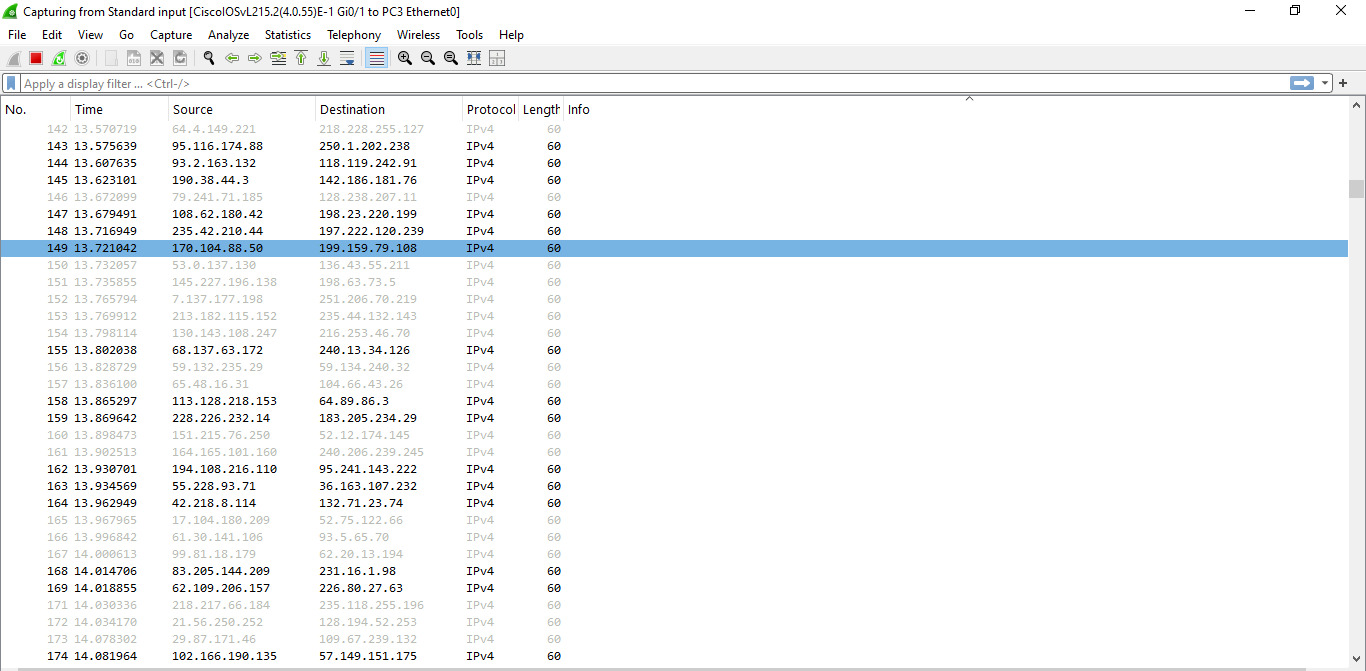
\includegraphics[width=1\linewidth]{../Images/wireshark1.jpeg}
    \caption{Wireshark capture during MAC table overflow attack}
    \label{fig:mac_overflow}
\end{figure}

\subsubsection{Switch Comparison}  

Cisco Catalyst 2960 supports port security, allowing the configuration of a maximum number of MAC addresses per port and defining actions when violations occur (e.g., restrict or shutdown). This makes it possible to prevent MAC table overflow attacks.

Link: \url{www.cisco.com/c/en/us/products/switches/catalyst-2960-series-switches/index.html}

\vspace{0.3cm}

In contrast, the TP-Link TL-SF1005D is an unmanaged switch that does not support port security or any traffic control mechanisms, as it lacks a configuration interface. Therefore, it cannot prevent MAC flooding attacks.

Link: \url{www.tp-link.com/en/home-networking/soho-switch/tl-sf1005d/}

\subsubsection{Feasibility}  
The objective of this attack is to flood the switch MAC address table, forcing the switch to behave like a hub. In that state, frames may be forwarded to all ports, allowing the attacker to listen to conversations between other hosts.

However, in practice, the attack may be difficult to execute successfully on modern switches because their MAC address tables are large. Additionally, the high amount of generated traffic can cause network instability or a denial-of-service condition, instead of allowing the attacker to reliably capture useful traffic.

Therefore, although the attack is theoretically possible, its practical feasibility is limited and depends on the switch capacity, configuration, and security features.

\subsection{DHCP spoofing}

\subsubsection{Attack and Countermeasure}  
The DHCP spoofing attack was performed by introducing a rogue DHCP server that responds to DHCP Discover messages with malicious configuration parameters.

As observed in Wireshark (Figure~\ref{fig:dhcp_attack}), multiple DHCP Offer messages were received for the same transaction ID, indicating a race condition between the legitimate and the rogue DHCP servers. The victim accepts the first Offer received, which may result in a malicious gateway configuration provided by the attacker.

\begin{figure}[h]
    \centering
    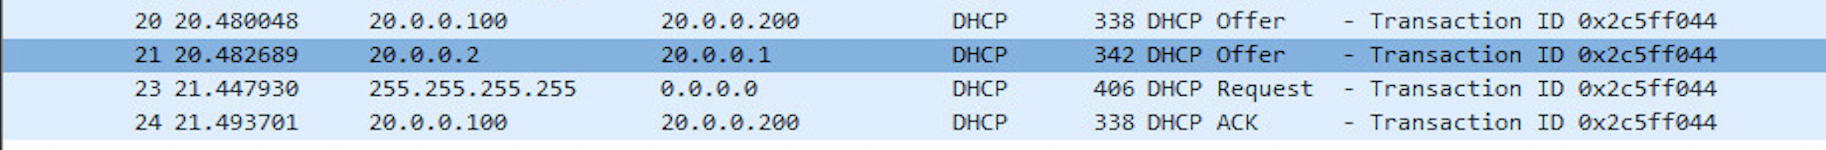
\includegraphics[width=1\linewidth]{../Images/wireshark2.png}
    \caption{Wireshark capture showing multiple DHCP Offer messages (attack)}
    \label{fig:dhcp_attack}
\end{figure}

After enabling DHCP snooping and configuring the port connected to the legitimate DHCP server as trusted, only one DHCP Offer was observed (Figure~\ref{fig:dhcp_snooping}). The rogue DHCP responses were blocked by the switch, and the client received a valid configuration. This confirms that DHCP snooping effectively mitigates the attack.

\begin{figure}[h]
    \centering
    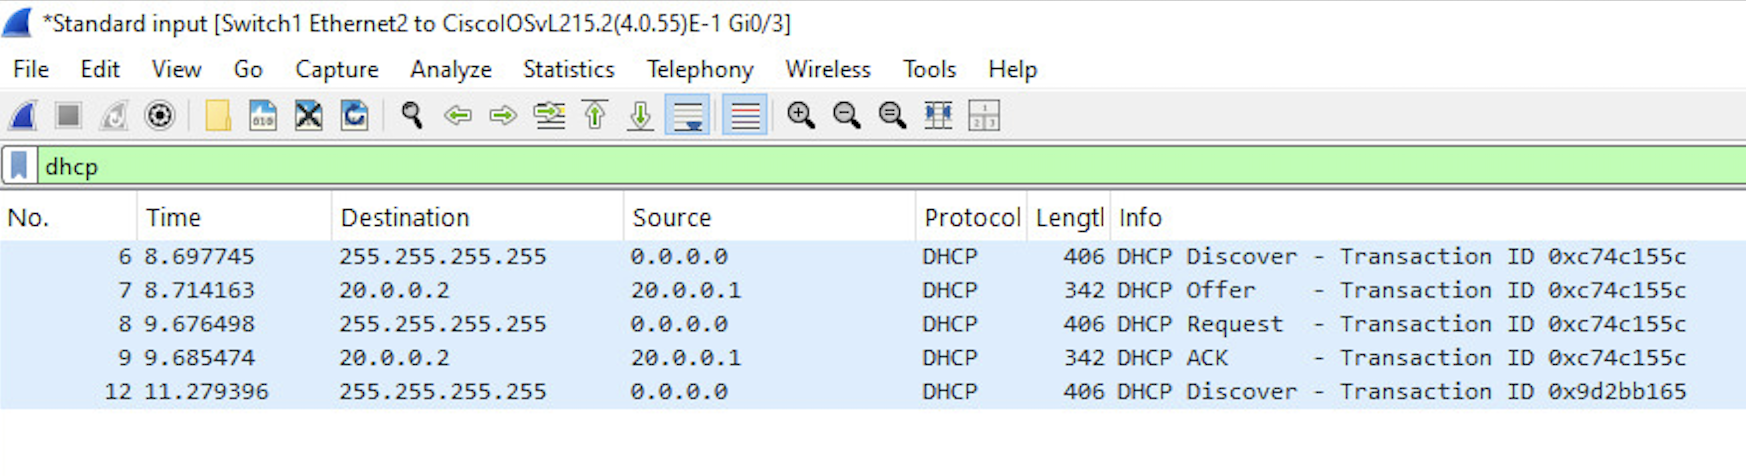
\includegraphics[width=1\linewidth]{../Images/wireshark3.png}
    \caption{Wireshark capture with DHCP snooping enabled (only legitimate Offer)}
    \label{fig:dhcp_snooping}
\end{figure}



\subsubsection{AI Prediction}  
The AI predicted that the victim closer to the attacker would be more likely to be compromised, since the rogue DHCP Offer would arrive first. This prediction matched the experimental results, where the victim receiving the first Offer obtained the malicious configuration.

\subsubsection{Switch Comparison}  
Cisco Catalyst 2960 supports DHCP snooping, allowing ports to be classified as trusted or untrusted and blocking DHCP server messages from untrusted ports.

Link: \url{www.cisco.com/c/en/us/products/switches/catalyst-2960-series-switches/index.html}

\vspace{0.3cm}

The TP-Link TL-SF1005D does not support DHCP snooping, as it is an unmanaged switch without configuration capabilities or security features.

Link: \url{www.tp-link.com/en/home-networking/soho-switch/tl-sf1005d/}

\subsubsection{Feasibility}  
The attack is feasible in networks without DHCP snooping, especially when the attacker is closer to the victim than the legitimate DHCP server. However, due to the race condition, success is not guaranteed. When DHCP snooping is enabled, the attack becomes ineffective.

\subsection{ARP poisoning (MitM)}

\subsubsection{Network Topology}  
The ARP poisoning attack was performed in the network shown in Figure~\ref{fig:arp_topology}, where two hosts communicate through a switch and an attacker is connected to the same Layer 2 domain.

\begin{figure}[H]
    \centering
    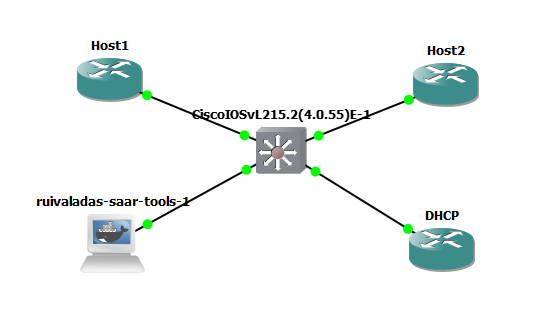
\includegraphics[width=0.6\linewidth]{../Images/topologiaARP.png}
    \caption{Network topology for ARP poisoning attack}
    \label{fig:arp_topology}
\end{figure}

\newpage

\subsubsection{Attack and Countermeasure}  

As observed in Wireshark (Figure~\ref{fig:arp_mitm}), ARP packets indicate duplicate IP usage, confirming that the attacker is associating its MAC address with multiple IP addresses.  

At the same time, ICMP traffic between the victims is still observed, which demonstrates that communication is maintained while being intercepted by the attacker, confirming a successful Man-in-the-Middle (MitM) condition.

\begin{figure}[H]
    \centering
    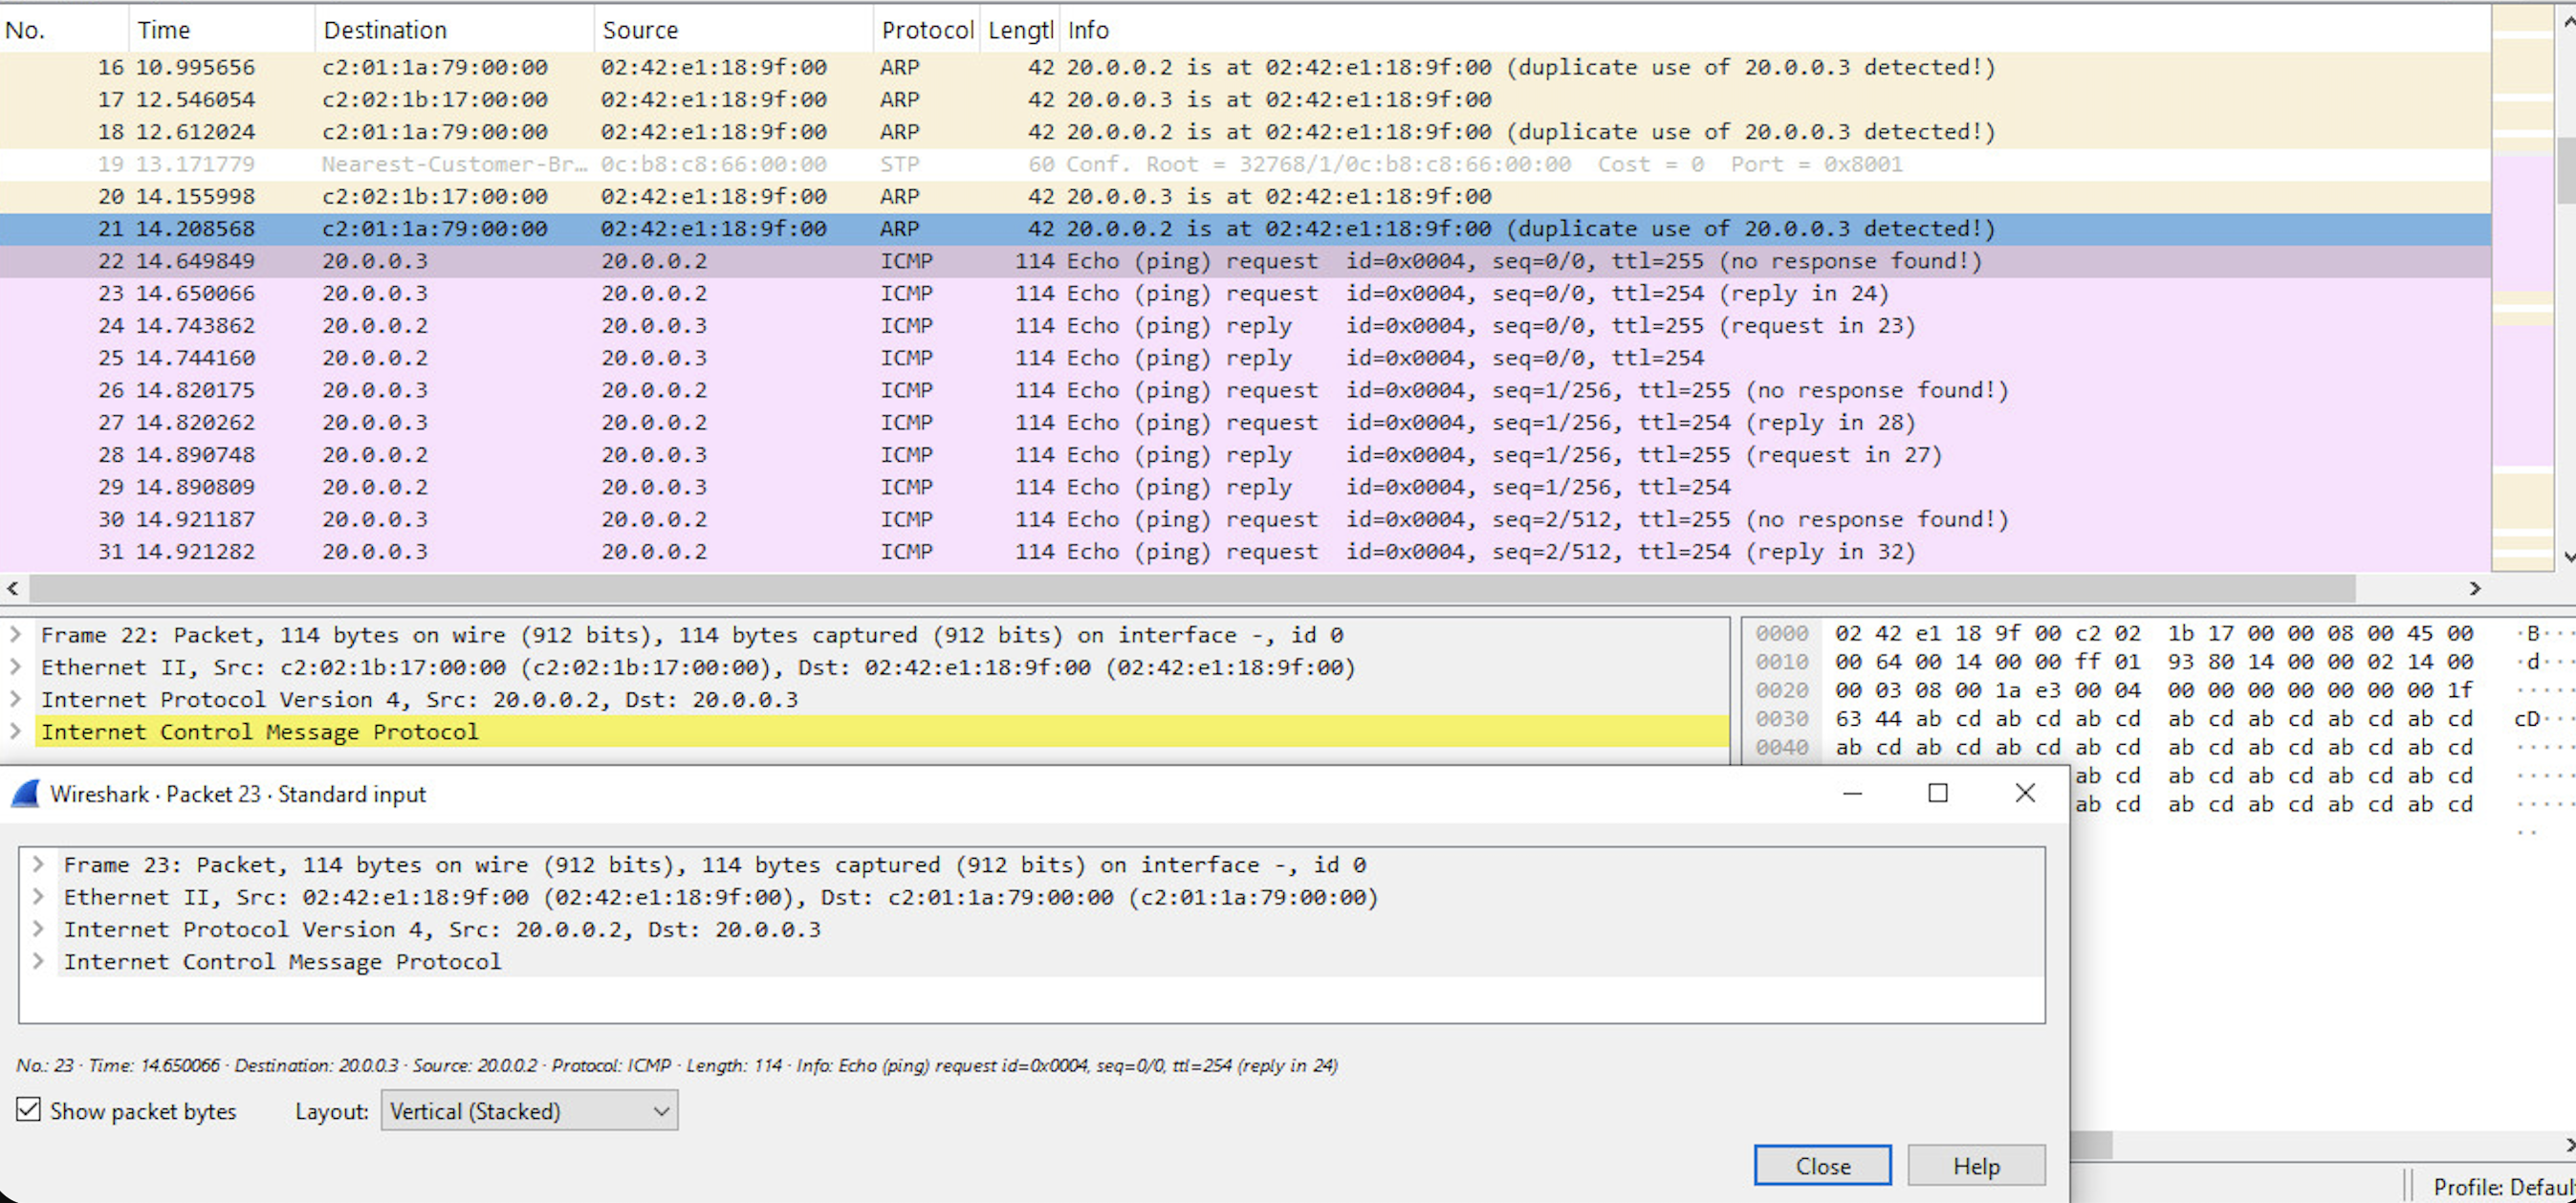
\includegraphics[width=0.9\linewidth]{../Images/ARPoison.png}
    \caption{ARP poisoning showing duplicate IP detection and intercepted ICMP traffic}
    \label{fig:arp_mitm}
\end{figure}

The attacker generated multiple forged ARP requests and replies, attempting to poison the ARP tables of the victims, as shown in Figure~\ref{fig:arp_attack}.

\begin{figure}[H]
    \centering
    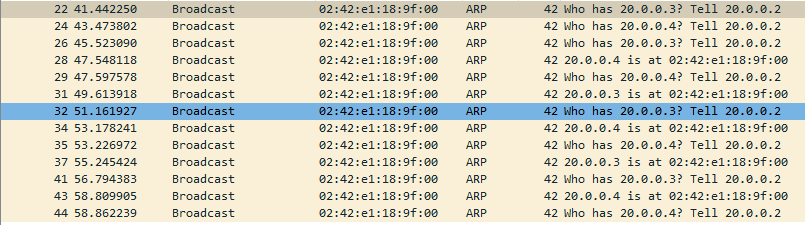
\includegraphics[width=0.9\linewidth]{../Images/blockedattacks.png}
    \caption{ARP packets generated by the attacker}
    \label{fig:arp_attack}
\end{figure}

However, the attack was mitigated using Dynamic ARP Inspection (DAI). The switch detected invalid ARP packets and blocked them, as shown in the system logs (Figure~\ref{fig:dai_log}).

\begin{figure}[H]
    \centering
    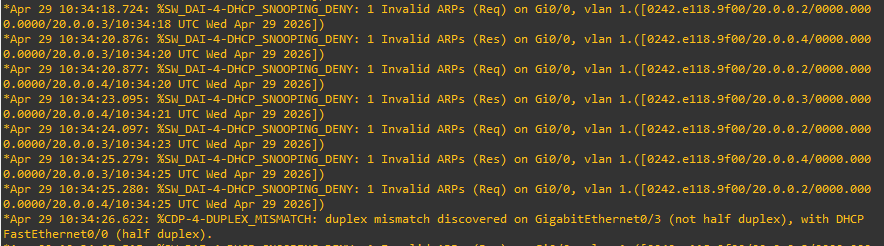
\includegraphics[width=0.9\linewidth]{../Images/logDAI.png}
    \caption{DAI log showing invalid ARP packets being denied}
    \label{fig:dai_log}
\end{figure}

\subsubsection{Defense Statistics}  
The effectiveness of DAI is confirmed by the statistics shown in Figure~\ref{fig:dai_stats}, where a high number of ARP packets were dropped by the switch.

\begin{figure}[H]
    \centering
    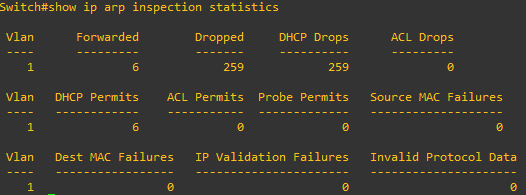
\includegraphics[width=0.7\linewidth]{../Images/defencestats.png}
    \caption{DAI statistics showing dropped ARP packets}
    \label{fig:dai_stats}
\end{figure}

\vspace{0.3cm}

\subsubsection{AI Configuration vs Experimental Setup}  
The AI suggested enabling DHCP snooping and configuring Dynamic ARP Inspection on the switch, marking trusted interfaces accordingly.  

This matched the experimental setup, where DHCP snooping was required for DAI to validate ARP packets. The configuration had to be adapted to the topology, particularly in defining trusted ports and VLAN configuration.

\vspace{0.3cm}

\subsubsection{Switch Comparison}  
Cisco Catalyst 2960 supports Dynamic ARP Inspection, allowing validation of ARP packets based on DHCP snooping bindings.

Link: \url{www.cisco.com/c/en/us/products/switches/catalyst-2960-series-switches/index.html}

The TP-Link TL-SF1005D does not support DAI, as it is an unmanaged switch without security or inspection mechanisms.

Link: \url{www.tp-link.com/en/home-networking/soho-switch/tl-sf1005d/}

\vspace{0.3cm}

\subsubsection{Feasibility}  
The attacker attempted to poison the ARP tables by sending forged ARP messages. The attack successfully created a Man-in-the-Middle condition, as observed in Wireshark. However, based on the switch logs and DAI statistics, these packets were detected and blocked.

Therefore, although the attack is feasible in networks without protection, in this setup it was not successful due to the correct configuration of Dynamic ARP Inspection.

\subsection{DNS spoofing}

\subsubsection{Attack Description}

The attack combined ARP poisoning with DNS spoofing
to redirect the victim's traffic to a malicious host.

Initially, the attacker poisoned the ARP caches
of the victim and the gateway by repeatedly sending
forged ARP replies claiming ownership of multiple IP addresses.

As a result, the victim associated the attacker's MAC address
with the IP addresses of legitimate hosts on the network,
allowing the attacker to position itself as a man-in-the-middle.

After intercepting the traffic, the attacker responded
to DNS queries with forged DNS responses containing
malicious IP addresses.

The victim then attempted to establish TCP/TLS connections
towards the attacker-controlled destination instead
of the legitimate server.

\subsubsection{Analysis of ARP, DNS and TCP Packets}

The attack started with ARP poisoning packets used
to manipulate the victim's ARP cache.

Once positioned as a man-in-the-middle,
the attacker intercepted DNS requests and generated
forged DNS replies redirecting the victim to a malicious IP address.

The victim then attempted to establish TCP/TLS connections
towards the spoofed destination.

The Wireshark captures show the full sequence of events:

\begin{enumerate}
\item Forged ARP replies poison the ARP cache
\item DNS requests are intercepted
\item Spoofed DNS replies redirect the victim
\item TCP/TLS connections are attempted
\item TLS communication fails due to certificate mismatch
\end{enumerate}

\begin{figure}[H]
\centering
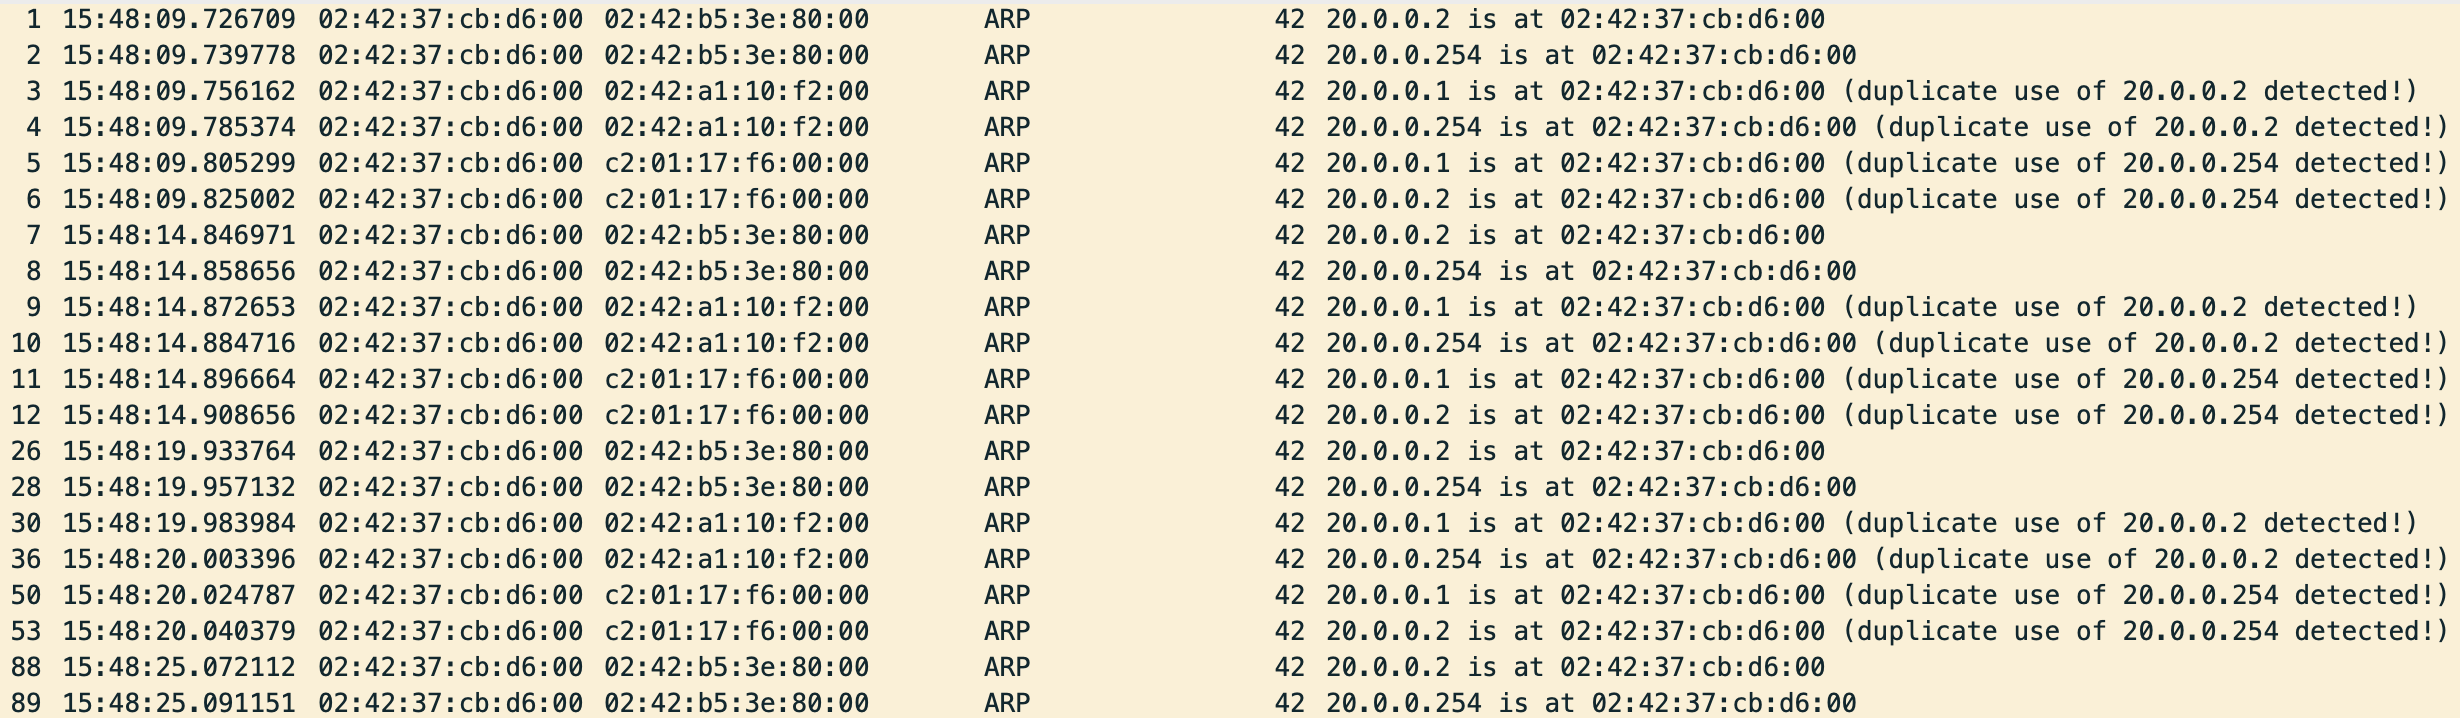
\includegraphics[width=\textwidth]{../Images/arp_poisoning.png}
\caption{Wireshark capture showing repeated forged ARP replies}
\label{fig:arp-poisoning}
\end{figure}

The ARP capture shows multiple unsolicited ARP replies
claiming that several IP addresses correspond to
the same MAC address.

Messages such as:

\begin{configbox}
20.0.0.2 is at 02:42:37:cb:d6:00
20.0.0.254 is at 02:42:37:cb:d6:00
\end{configbox}

indicate that the attacker continuously poisoned
the ARP caches of the victim and gateway.

Wireshark also detected duplicate IP usage warnings,
which is a strong indication of ARP spoofing activity.

\begin{figure}[H]
\centering
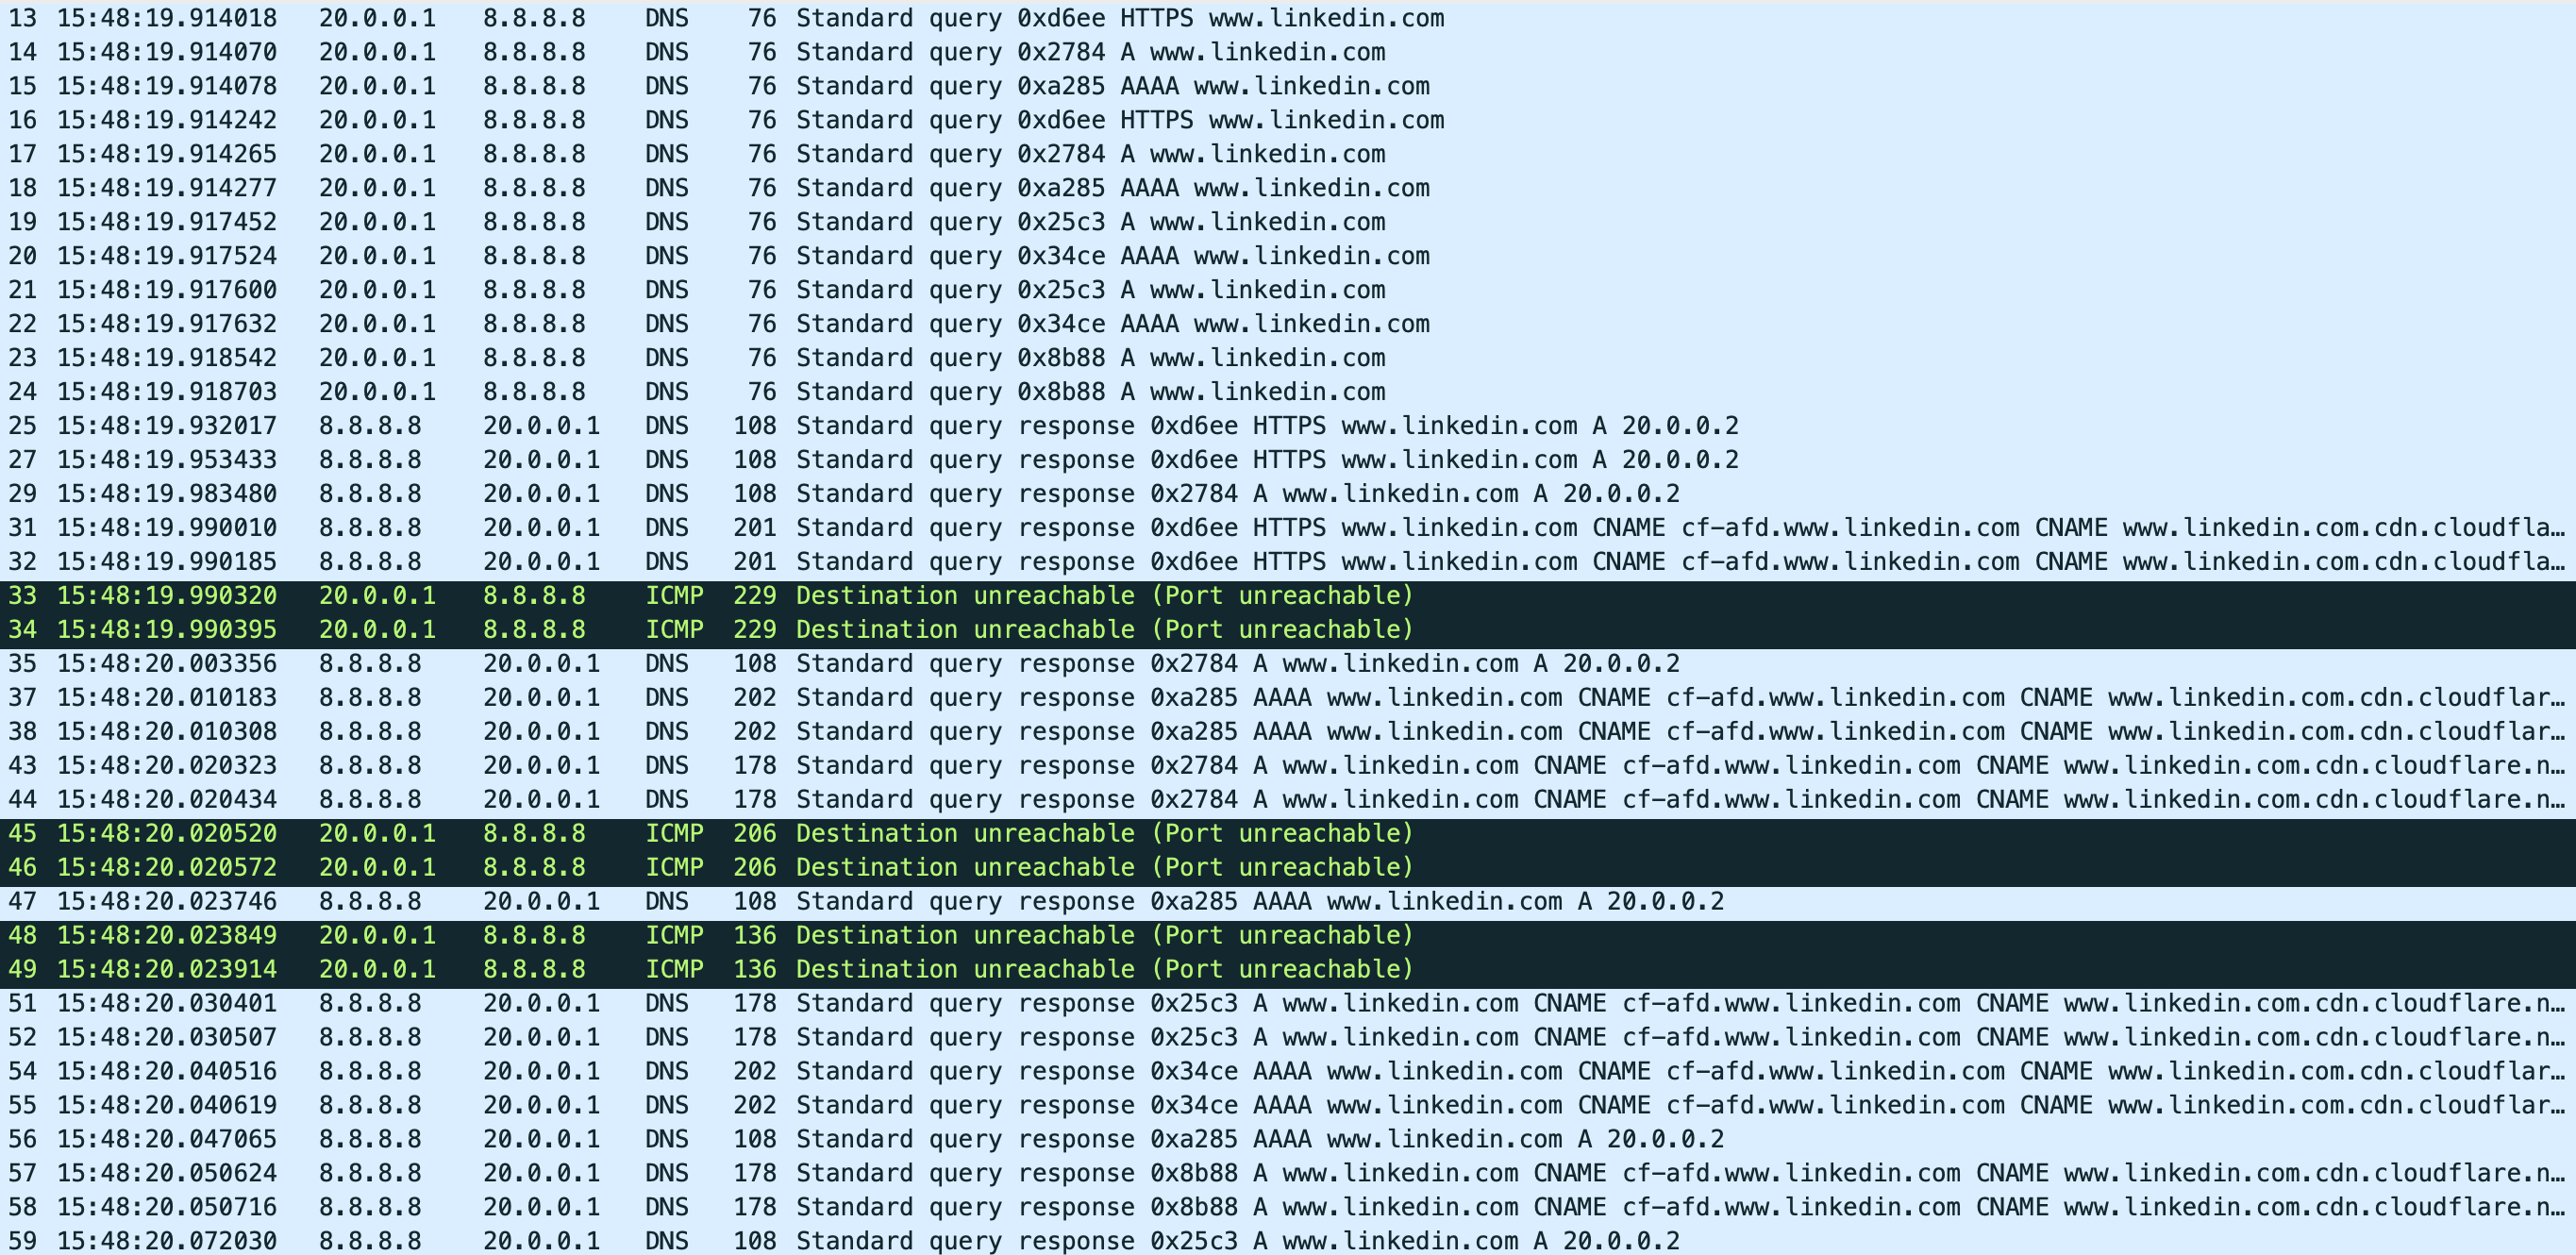
\includegraphics[width=\textwidth]{../Images/dns_spoofing2.png}
\caption{Forged DNS responses observed in Wireshark}
\label{fig:dns-spoofing}
\end{figure}

The DNS capture shows queries for the domain
\texttt{www.linkedin.com} followed by forged DNS responses.

Instead of returning the legitimate public IP address,
the spoofed DNS responses mapped the domain name
to the malicious local IP address:

\begin{configbox}
www.linkedin.com A 20.0.0.2
\end{configbox}

This demonstrates that the attacker successfully
intercepted and manipulated DNS traffic.

\begin{figure}[H]
\centering
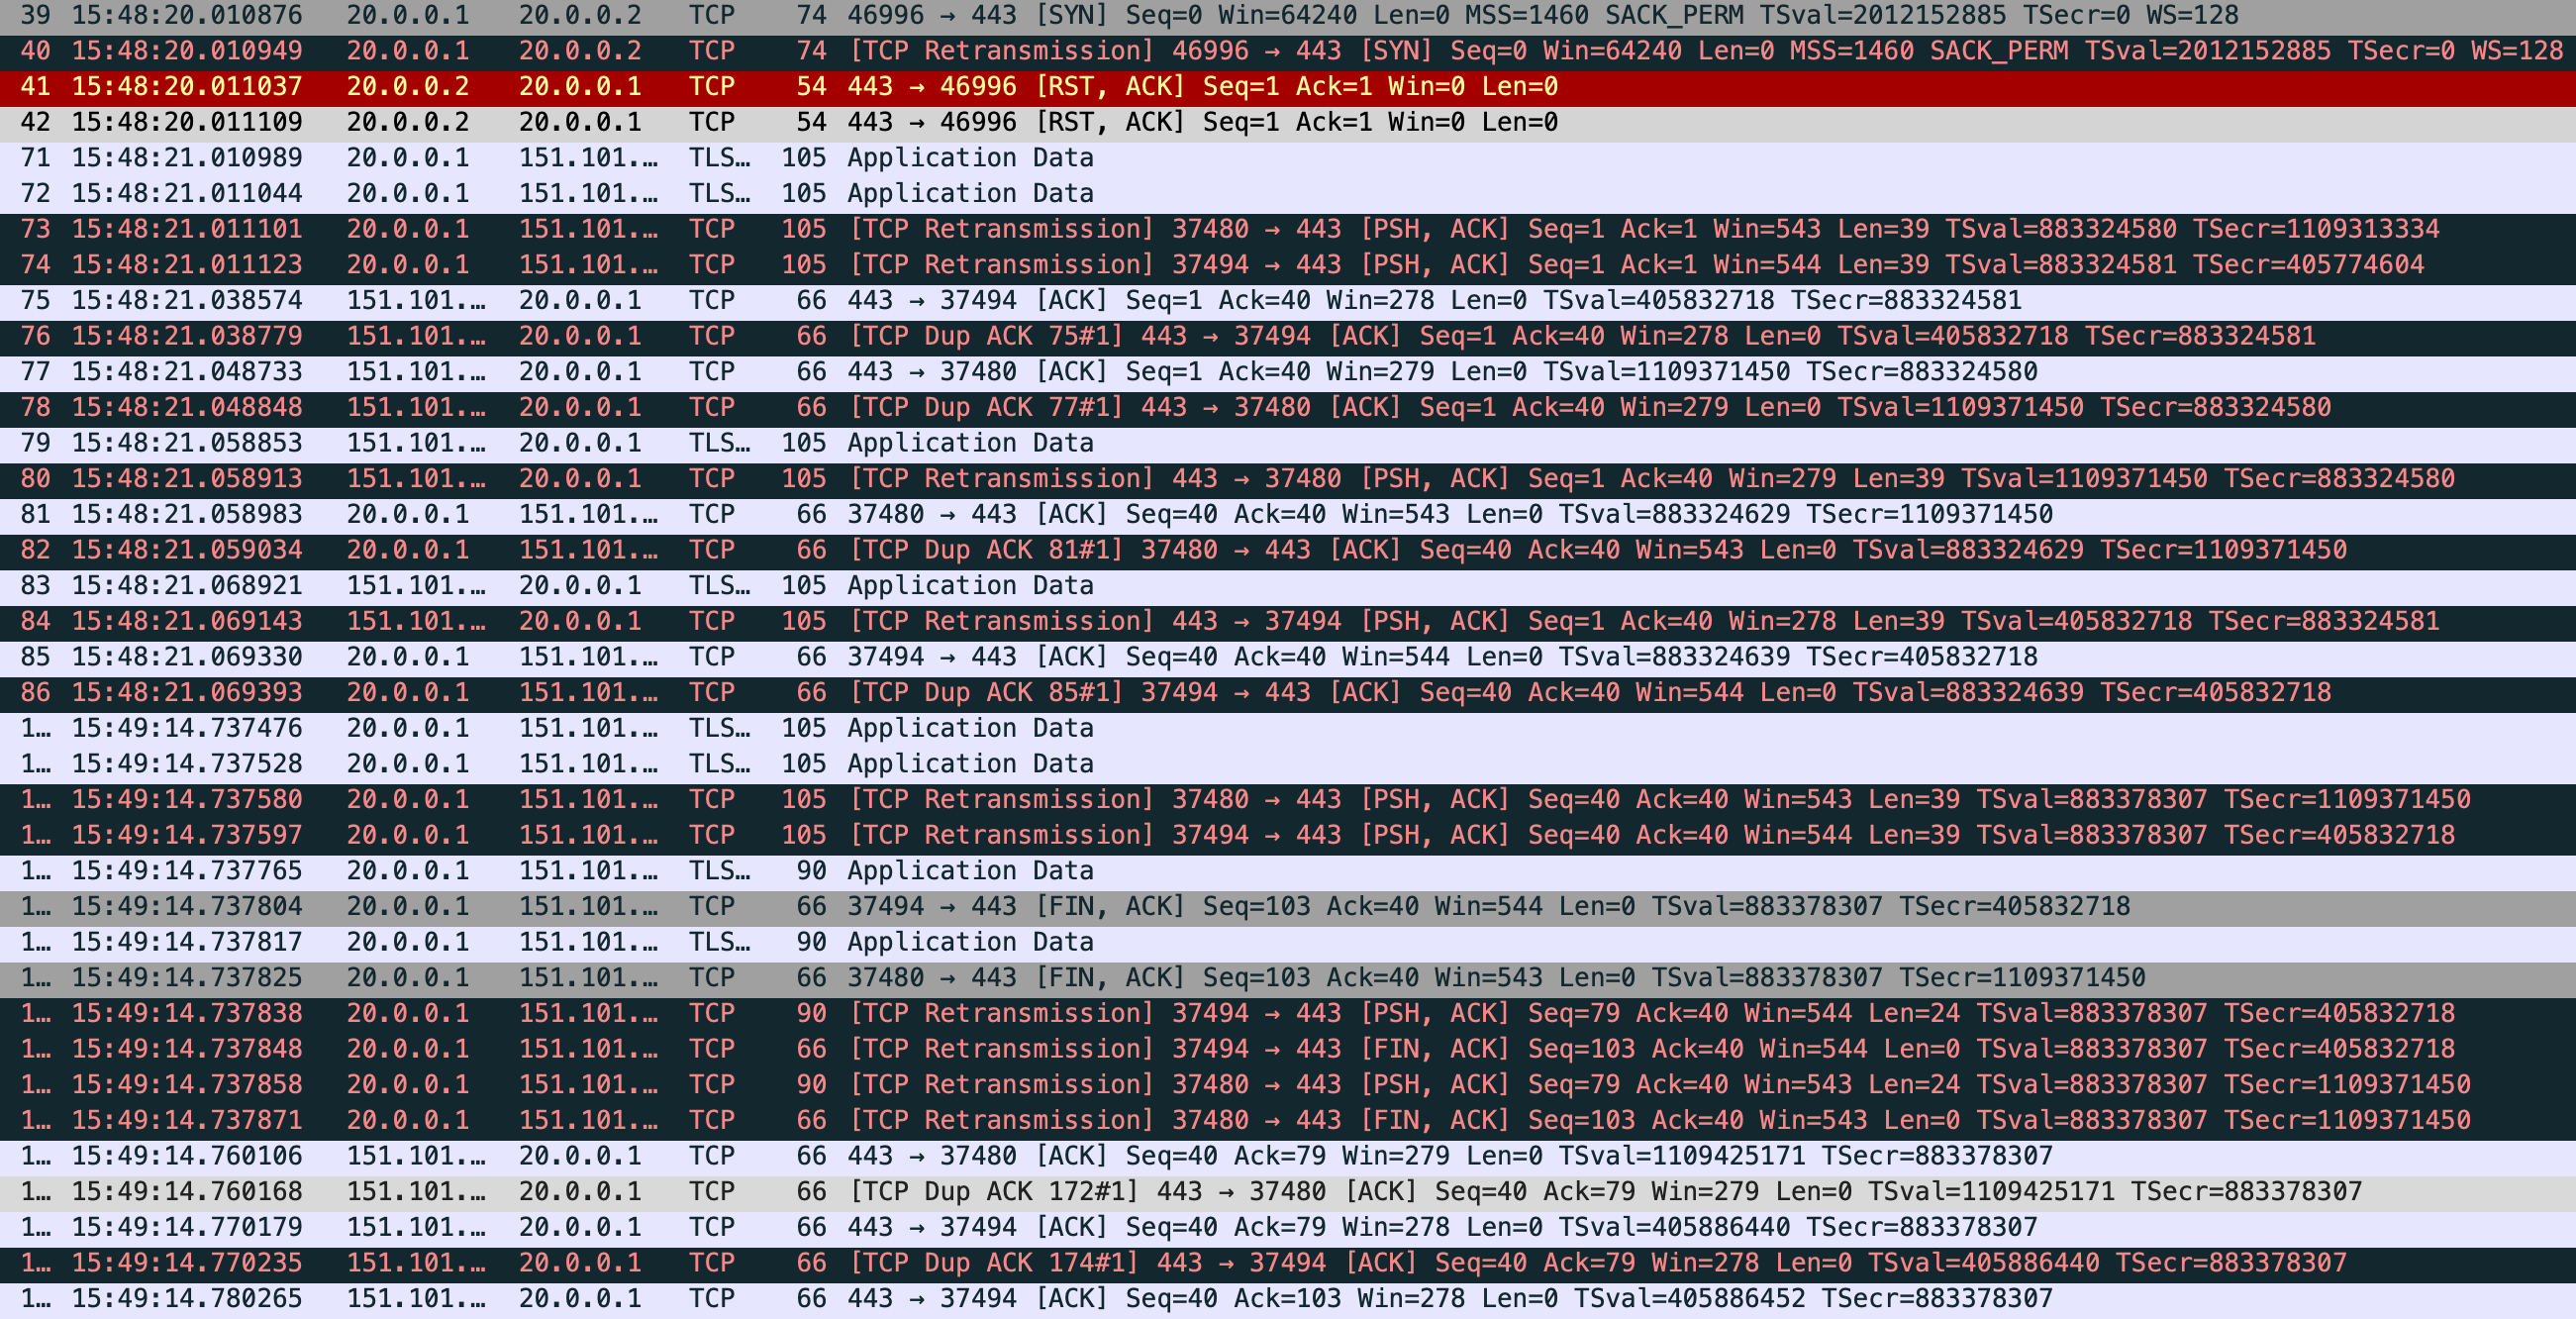
\includegraphics[width=\textwidth]{../Images/tcp_tls_failure.png}
\caption{TCP and TLS communication after DNS spoofing}
\label{fig:tcp-tls}
\end{figure}

After the spoofed DNS resolution, the victim attempted
to establish TCP and TLS sessions with the attacker-controlled host.

However, the packet capture shows multiple TCP retransmissions,
duplicate acknowledgements, and TCP reset packets.

This behavior indicates that the TLS session could not
be properly established.

The failure likely occurred because the attacker did not possess
a valid TLS certificate for the spoofed domain,
causing the browser or TLS stack to reject the connection.

\subsubsection{AI Explanation and Experimental Comparison}

An AI-generated explanation suggested that DNS spoofing
may fail even when ARP poisoning is successful because
modern browsers and operating systems implement additional
security mechanisms such as:

\begin{itemize}
\item DNS caching
\item HTTPS and TLS certificate validation
\item HSTS policies
\item DNS-over-HTTPS (DoH)
\item Browser security protections
\end{itemize}

The experimental observations largely matched this explanation.

Although ARP poisoning was clearly successful,
as demonstrated by the repeated forged ARP replies,
the final TCP/TLS communication did not fully succeed.

The Wireshark captures show TCP retransmissions,
duplicate ACKs, and TCP reset packets after the spoofed DNS replies.

This suggests that the victim attempted to establish
a secure HTTPS connection but rejected the spoofed server
because it could not provide a valid TLS certificate
for the requested domain.

Therefore, the experiment confirms that successful ARP poisoning
alone does not guarantee successful DNS spoofing attacks
against modern HTTPS-protected services.

The roles of the entities involved in the authentication process
were also correctly explained by the AI tool:

\begin{itemize}
\item The victim host acted as the DNS client
\item The attacker acted as a man-in-the-middle
through ARP poisoning
\item The DNS server was impersonated through forged responses
\end{itemize}

These behaviors were directly observable in the packet captures.

\subsubsection{Feasibility of the Attack}

The experiment demonstrates that ARP poisoning
and DNS spoofing attacks are technically feasible
in local networks where hosts trust ARP replies
without authentication.

However, the practical effectiveness of the attack
against modern websites is significantly reduced
by HTTPS and TLS protections.

Even though DNS manipulation succeeded,
the browser and TLS mechanisms prevented
the attacker from fully impersonating
the legitimate website.

The attack would be significantly more effective
against:

\begin{itemize}
\item Unencrypted HTTP services
\item Legacy devices
\item Misconfigured networks
\item Users ignoring TLS certificate warnings
\end{itemize}

\subsubsection{Countermeasures}

Several mechanisms can mitigate ARP poisoning
and DNS spoofing attacks:

\begin{itemize}
\item Static ARP entries
\item Dynamic ARP Inspection (DAI)
\item DHCP Snooping
\item DNSSEC
\item HTTPS and TLS certificate validation
\item HSTS
\item VPN usage
\item Network segmentation
\item Intrusion detection systems
\end{itemize}

Modern HTTPS deployments significantly reduce
the effectiveness of DNS spoofing attacks,
since attackers cannot easily present valid
TLS certificates for legitimate domains.


\subsection{RIP Poisoning}

\subsubsection{Network Topology}

The RIP poisoning attack was performed using the topology shown in Figure~\ref{fig:rip_topology}. The Web browser, the legitimate Web server and the fake Web server are located in different subnets, with the attacker collocated with the fake Web server.

\begin{figure}[H]
    \centering
    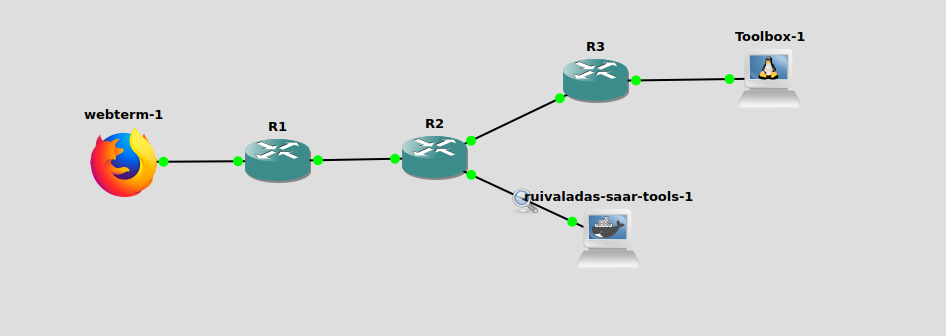
\includegraphics[width=0.9\linewidth]{../Images/topologyRIPoisoning.png}
    \caption{Network topology used for the RIP poisoning attack}
    \label{fig:rip_topology}
\end{figure}

\subsubsection{Attack and Countermeasure}

The attacker sent forged RIPv2 Response messages in order to poison the routing tables of the routers. These messages advertised a route to the legitimate Web server network through the attacker, causing traffic from the browser to be redirected to the fake Web server.

As shown in Figure~\ref{fig:rip_packets}, Wireshark captured multiple RIPv2 Response packets sent to the multicast address \texttt{224.0.0.9}, which is used by RIPv2 routers. The captured packet advertises the network \texttt{10.0.0.0} with metric 5 and subnet mask \texttt{255.255.255.128}, showing that the attacker injected routing information into the network.

\begin{figure}[H]
    \centering
    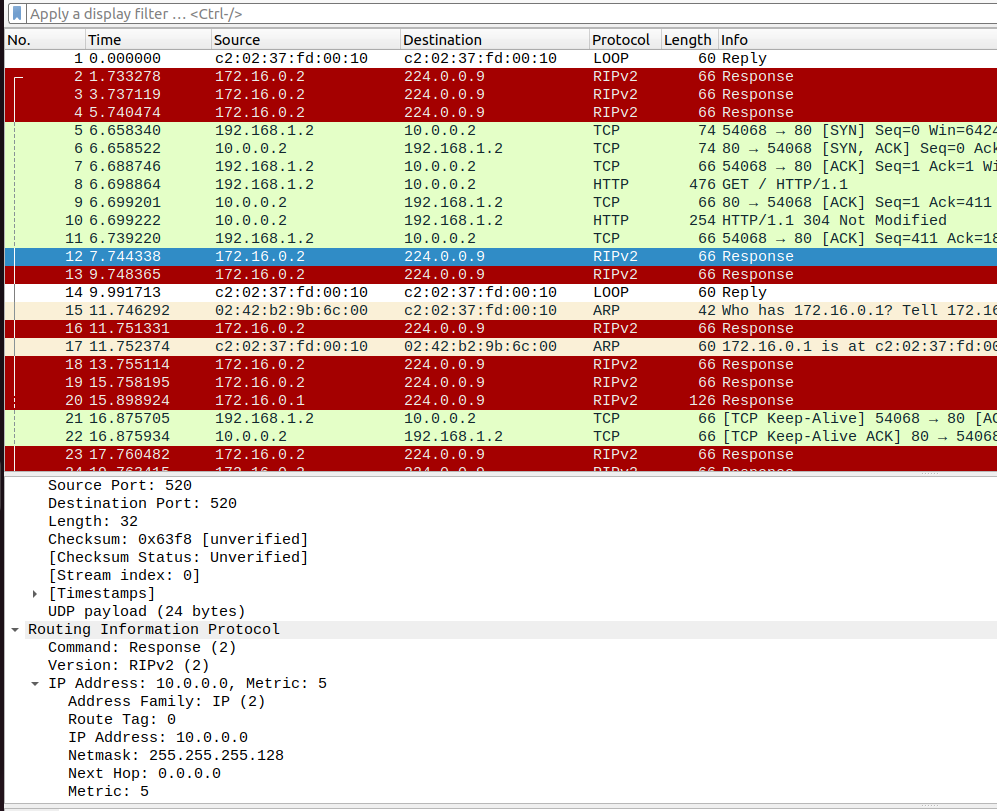
\includegraphics[width=0.9\linewidth]{../Images/RIPoisoning1.png}
    \caption{Forged RIPv2 response advertising a route to the target network}
    \label{fig:rip_packets}
\end{figure}

The effect of the attack was confirmed in the browser. As shown in Figure~\ref{fig:rip_fake_server}, the Web browser was redirected to the fake Web server, displaying the message \textit{``FAKE SERVER - ATTACK SUCCESS''}.

\vspace{0.3cm}

\begin{figure}[H]
    \centering
    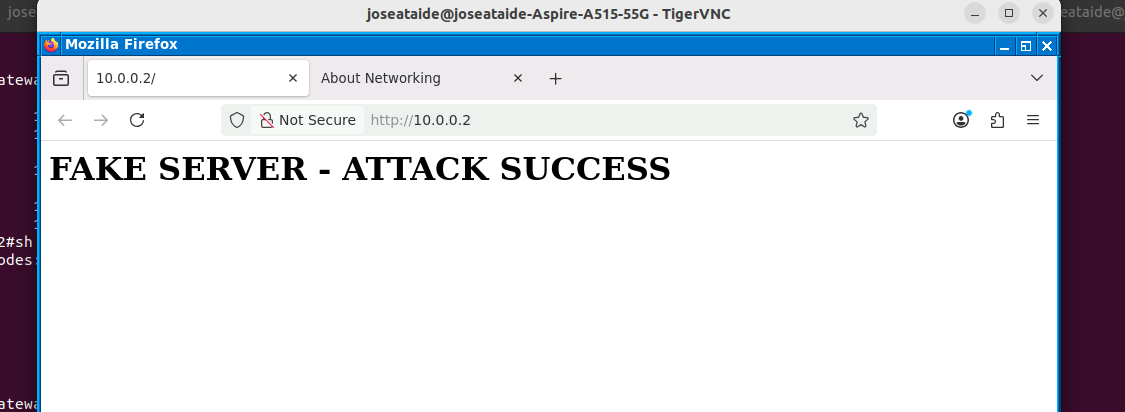
\includegraphics[width=0.9\linewidth]{../Images/RIPoisoning3.png}
    \caption{Browser redirected to the fake Web server}
    \label{fig:rip_fake_server}
\end{figure}

\newpage

Additional Wireshark captures show TCP and HTTP communication between the browser and the fake server, confirming that the traffic was redirected after the routing tables were poisoned.

\begin{figure}[H]
    \centering
    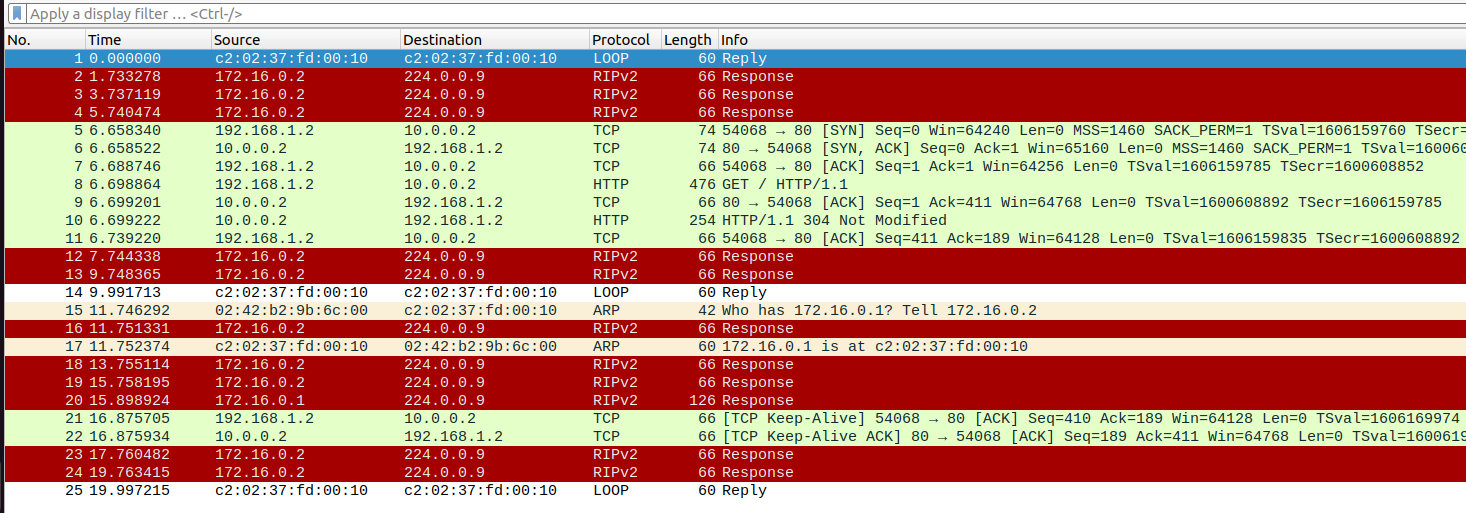
\includegraphics[width=0.9\linewidth]{../Images/RIPoisoning2.png}
    \caption{TCP and HTTP traffic redirected to the fake Web server}
    \label{fig:rip_tcp}
\end{figure}

As a countermeasure, RIPv2 authentication can be enabled on the routers. With authentication, routers only accept RIP updates from trusted devices, preventing forged routing updates from being installed in the routing table.

\subsubsection{Effectiveness of the Attack}

The success of the attack depends on the relative location of the browser, legitimate Web server and fake Web server. Since the attacker is placed near the fake Web server, it can advertise a route that makes the fake server appear as a better path to the target network.

The prefix length advertised by the attacker is also important. A more specific prefix is preferred due to the longest prefix match rule. Therefore, if the attacker advertises a more specific route than the legitimate one, the routers may select the malicious route.

RIP auto-summary can reduce the effectiveness of the attack because it summarizes routes at classful network boundaries. When auto-summary is disabled, more specific routes can be advertised, making the attack more effective.

Figures~\ref{fig:rip_filtered} and \ref{fig:rip_multicast} show repeated RIPv2 Response messages, confirming that the attacker continuously injected routing updates into the network.

\begin{figure}[H]
    \centering
    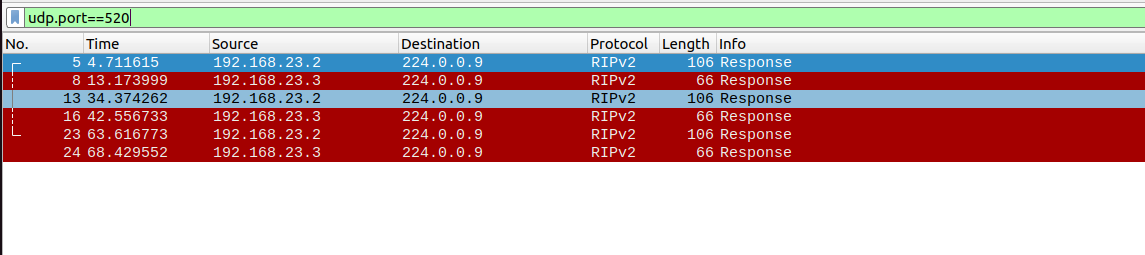
\includegraphics[width=0.9\linewidth]{../Images/RIPoisoning4.png}
    \caption{Filtered RIPv2 packets sent to multicast address 224.0.0.9}
    \label{fig:rip_filtered}
\end{figure}

\begin{figure}[H]
    \centering
    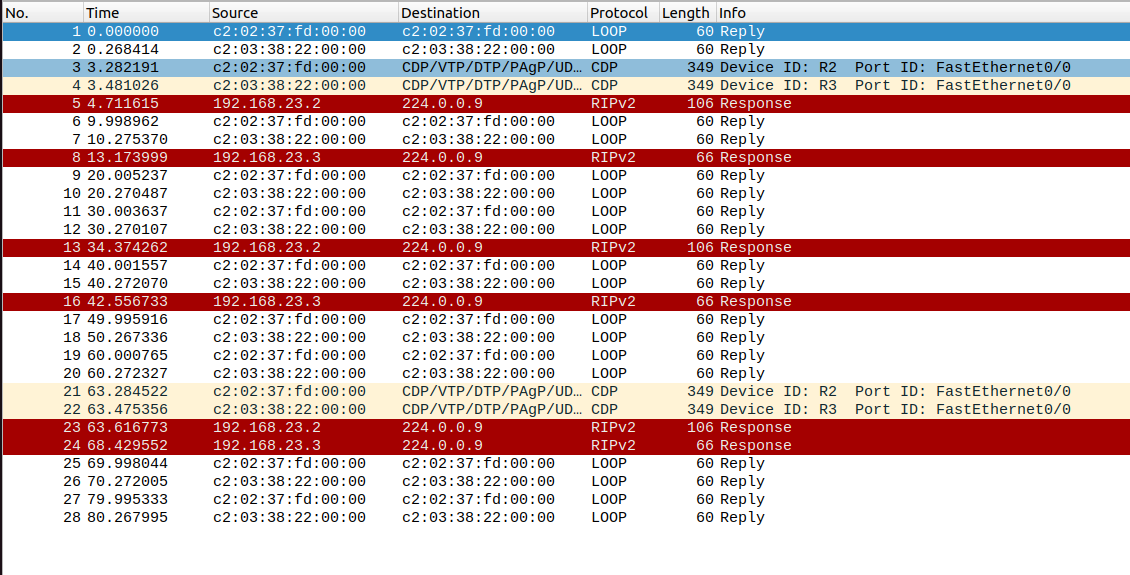
\includegraphics[width=0.9\linewidth]{../Images/RIPoisoning5.png}
    \caption{Repeated RIPv2 responses observed during the attack}
    \label{fig:rip_multicast}
\end{figure}

\subsubsection{AI Prediction vs Experimental Results}

The AI predicted that the attacker would be more successful when advertising a more specific prefix, because routers prefer the longest prefix match. It also predicted that disabling RIP auto-summary would make the attack more effective, since the malicious route would not be summarized.

This prediction matched the experimental behavior. The captured RIP packets show that the attacker advertised specific routing information, and the browser traffic was redirected to the fake Web server. Therefore, the observed results confirm that prefix length and auto-summary directly influence route selection.

\subsubsection{Feasibility}

This attack is feasible in networks using RIP without authentication. Since RIP accepts routing updates from neighboring devices, an attacker can inject forged routes and redirect traffic.

However, in modern networks, RIP is less common and authentication can prevent this attack. Therefore, the attack is mainly feasible in poorly configured or legacy networks.


%% DAQUI PARA BAIXO LAB 2 E 3

\newpage

\section {Firewalls}

\subsection{Classical firewalls versus Zone-Based Policy Firewalls}

\subsubsection{Firewall Validation}

The firewall must enforce the following rules:
\begin{enumerate}
    \item Block all traffic from INSIDE to OUTSIDE;
    \item Allow only ICMP and HTTP traffic from OUTSIDE to the server;
    \item Deny access to the firewall interfaces.
\end{enumerate}

\subsubsection{Classical Firewall (CBAC)}

In the classical firewall, traffic filtering is based on ACLs combined with stateful inspection rules. As shown in the slides, inspection rules only track sessions and do not impose restrictions by themselves.

Initially, the configuration allowed access to multiple server ports because the ACL was too permissive. This confirms that \textbf{inspect rules do not have an implicit deny}, meaning that unwanted traffic may still pass if not explicitly blocked.

After correcting the ACLs, the observed behavior was:
\begin{enumerate}
    \item Only HTTP and ICMP traffic to the server was allowed;
    \item All other ports were classified as filtered by NMAP;
    \item No traffic from INSIDE to OUTSIDE was possible due to explicit deny rules.
\end{enumerate}

\subsubsection{ZBPF}

In ZBPF, interfaces are assigned to zones and policies are applied between zones. By default, traffic between different zones is dropped unless a policy is defined.

After configuration, the firewall behavior was:
\begin{enumerate}
    \item Only explicitly permitted traffic (HTTP and ICMP to the server) was allowed;
    \item All other inter-zone traffic was blocked by default;
    \item Access to firewall interfaces was denied (controlled via the self zone).
\end{enumerate}

Therefore, both firewalls satisfy the specification, but ZBPF enforces it more naturally due to its default deny model.

\newpage

\subsection{NMAP Operation}

NMAP is used to discover hosts and scan ports by actively probing the network.

\subsubsection{Host Discovery}

When using \texttt{nmap -sn}, NMAP determines if hosts are active by sending:
\begin{enumerate}
    \item ICMP Echo requests;
    \item TCP SYN packets to common ports (e.g., port 80);
    \item ARP requests in local networks.
\end{enumerate}

A host is considered active if it replies to any of these probes.

\subsubsection{Port Scanning}

For port scanning, NMAP typically uses a TCP SYN scan:
\begin{enumerate}
    \item SYN-ACK response $\Rightarrow$ port is open;
    \item RST response $\Rightarrow$ port is closed;
    \item No response or ICMP error $\Rightarrow$ port is filtered.
\end{enumerate}

This method is efficient because it does not complete the TCP connection, allowing fast scanning of multiple ports.

\subsection{CBAC vs ZBPF}

The main differences between CBAC and ZBPF are:

\begin{enumerate}
    \item \textbf{Configuration model:}  
    CBAC is interface-based and relies on ACLs plus inspection rules, while ZBPF is zone-based and uses zone-pairs, class-maps, and policy-maps.

    \item \textbf{Default behavior:}  
    In CBAC, traffic may be allowed unless explicitly denied by ACLs. In ZBPF, traffic between zones is denied by default unless a policy allows it.

    \item \textbf{Stateful inspection:}  
    Both support stateful inspection, but in CBAC it depends on inspect rules applied to interfaces, whereas in ZBPF it is integrated into policy actions (inspect, pass, drop).

    \item \textbf{Security and control:}  
    ZBPF provides stricter and more modular control, since all inter-zone traffic must be explicitly defined. CBAC is less structured and more prone to configuration errors.
\end{enumerate}

In conclusion, although both approaches can enforce the required policy, ZBPF offers a more robust, scalable, and secure solution.

\newpage

\subsection{Protecting a Campus Network using ZBPF}

\subsubsection{Network Topology}

The network is divided into four security zones: PR1, PR2, DMZ, and OUT, as shown in Figure~\ref{fig:zbpf_topology}.  

The firewall is implemented on a Cisco 7200 router using Zone-Based Policy Firewall (ZBPF). The DMZ contains Web, Email, and DNS servers, while PR1 and PR2 represent private networks.

\begin{figure}[H]
    \centering
    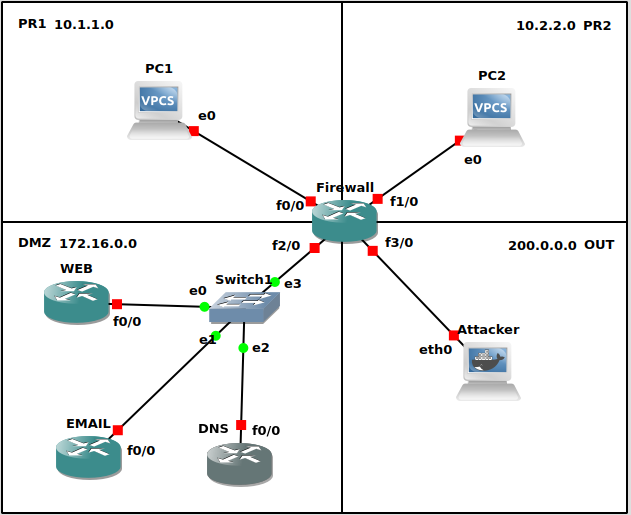
\includegraphics[width=0.8\textwidth]{../Images/topo_firewalls2.png}
    \caption{Campus network protected by a ZBPF firewall}
    \label{fig:zbpf_topology}
\end{figure}

\subsubsection{Firewall Configuration}

Four security zones were created and associated with the firewall interfaces. By default, communication between zones is denied unless explicitly permitted.

NAT overload was configured to allow private hosts to access the OUT zone while hiding internal IP addresses.

Traffic policies were implemented using ACLs, class-maps, policy-maps, and zone-pairs. Only the required services were allowed:
\begin{itemize}
    \item HTTP/HTTPS to the Web server;
    \item SMTP to the Email server;
    \item DNS queries to the DNS server.
\end{itemize}

No zone-pairs were configured between PR1 and PR2, nor from OUT towards the private zones, resulting in implicit traffic denial.

\subsubsection{Testing and Validation}

The firewall policies were validated using NMAP and Wireshark.

\paragraph{PR1 to PR2}

Communication between private zones was blocked. NMAP scans returned no responses, confirming inter-zone isolation.

\begin{figure}[H]
    \centering
    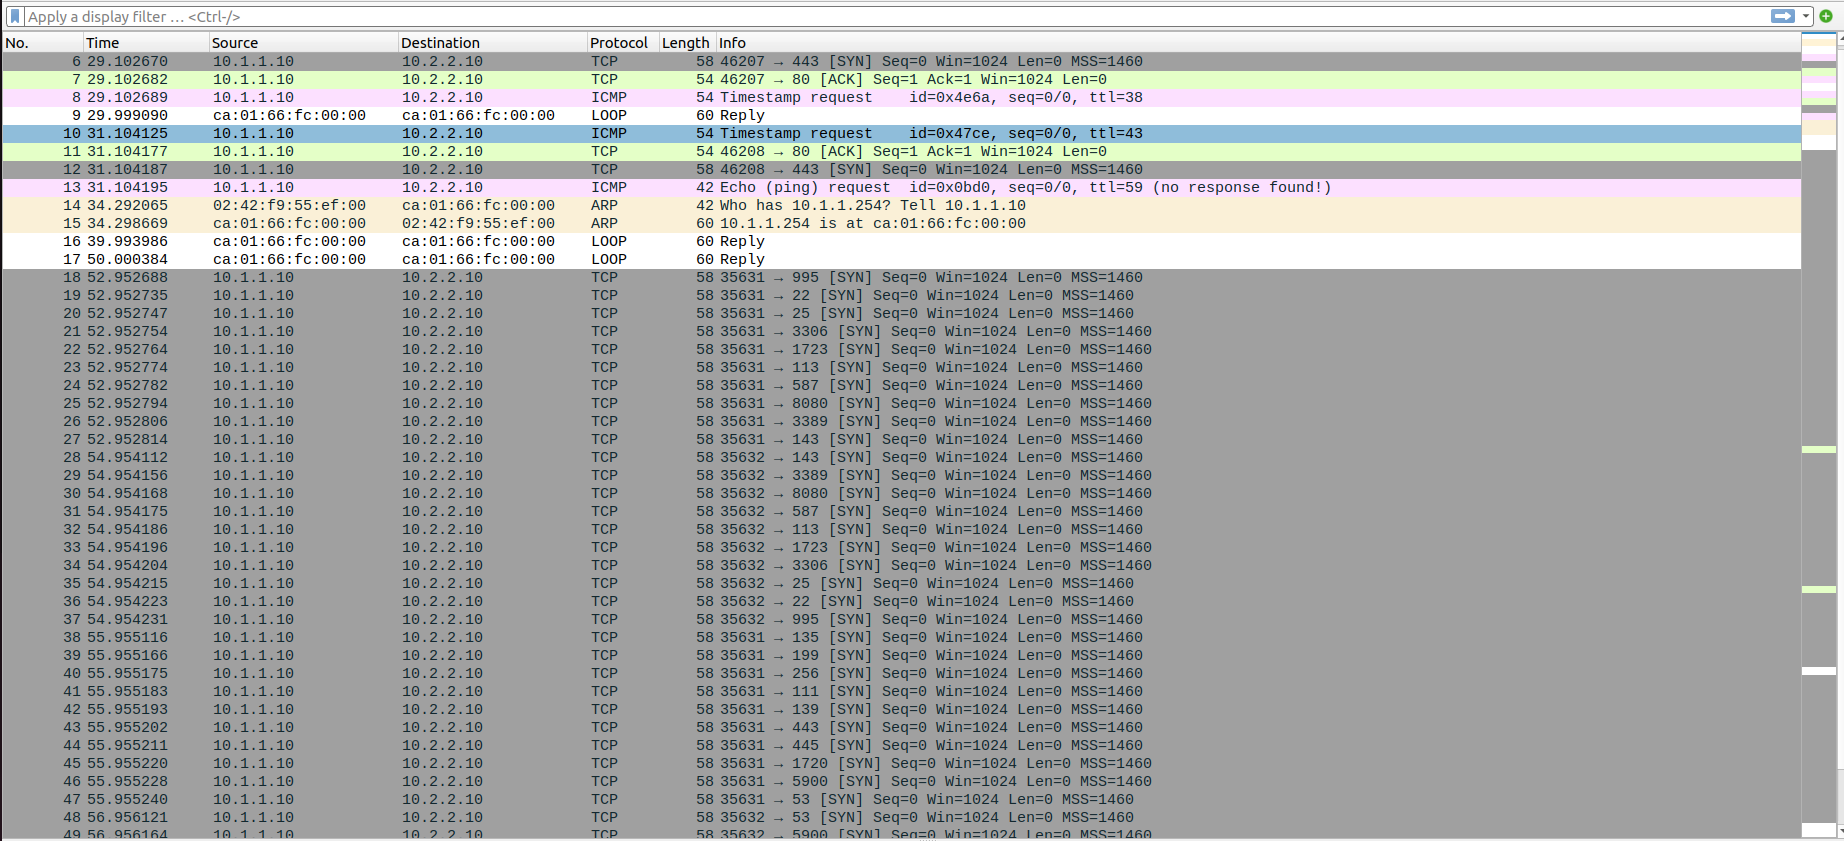
\includegraphics[width=1\linewidth]{../Images/Nmap_PR_to_PR(no replies).png}
    \caption{NMAP scan from PR1 to PR2 showing no replies, confirming inter-zone isolation enforced by the firewall}
    \label{fig:pr1_pr2_block}
\end{figure}

\paragraph{PR1 to OUT}

NAT operation was validated by scanning external hosts. Wireshark captures confirmed source address translation using the firewall public IP.

\begin{figure}[H]
    \centering
    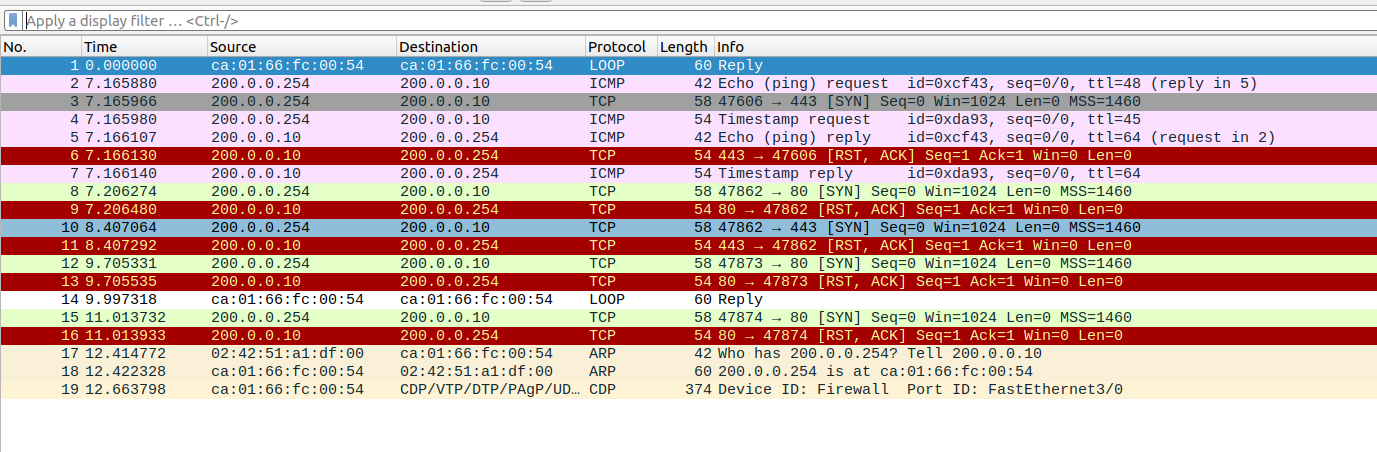
\includegraphics[width=1\linewidth]{../Images/Nmap_PR_to_OUT(NAT proof).png}
    \caption{Traffic from PR1 to the OUT zone showing NAT translation and access only to permitted services}
    \label{fig:nat_validation}
\end{figure}

\paragraph{PR1 to DMZ}

Only HTTP and HTTPS services were reachable on the DMZ Web server, while all other ports were filtered.

\begin{figure}[H]
    \centering
    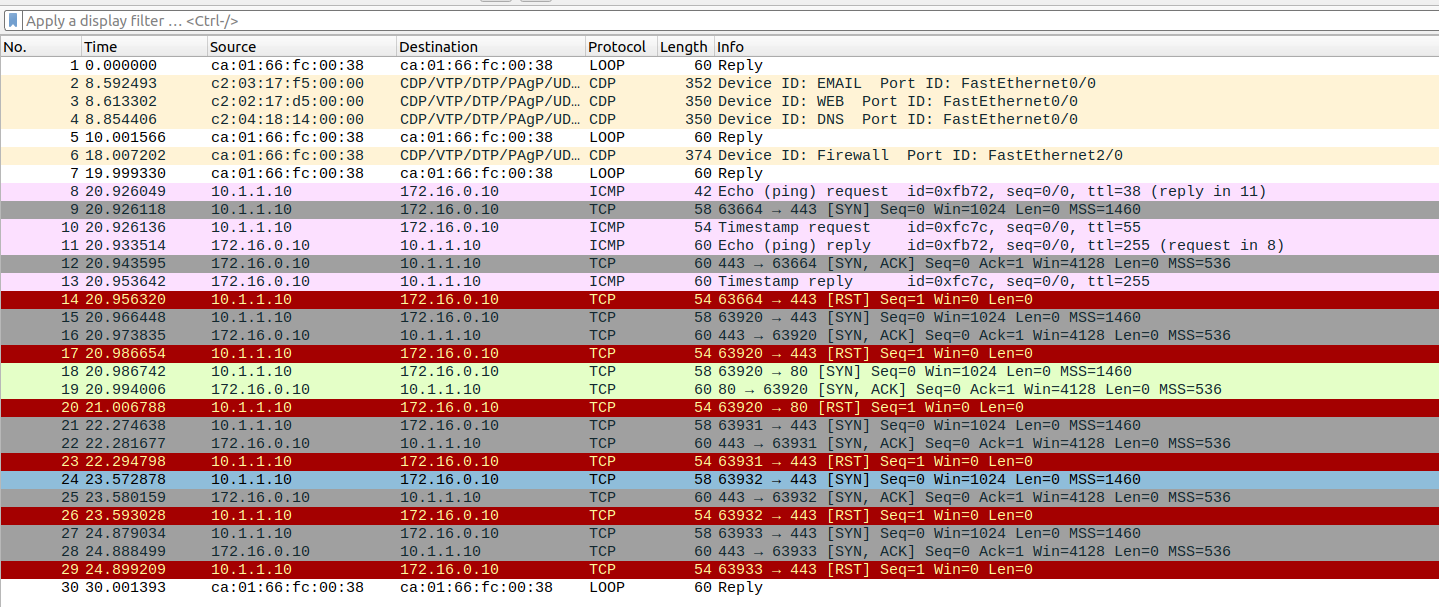
\includegraphics[width=1\linewidth]{../Images/nmap_PR_to_DMZ(working proof).png}
    \caption{NMAP scan from PR1 to the DMZ showing only HTTP and HTTPS services accessible}
    \label{fig:pr1_dmz}
\end{figure}

\paragraph{OUT to Private Zones}

Connections from the OUT zone to PR1 and PR2 were unsuccessful, confirming that private networks are protected from external access.

\paragraph{OUT to DMZ}

Only the permitted public services were accessible from the OUT zone.

\begin{figure}[H]
    \centering
    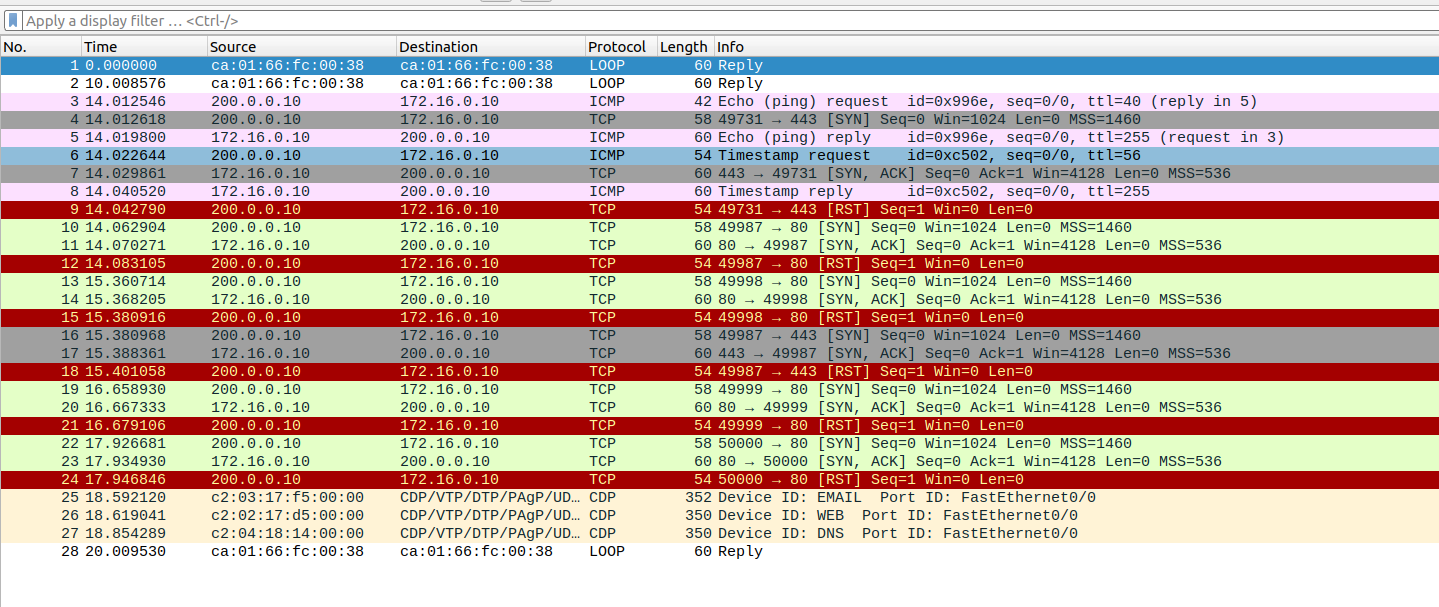
\includegraphics[width=1\linewidth]{../Images/nmap_OUT_to_DMZ.png}
    \caption{Access from the OUT zone to the DMZ restricted to publicly allowed services}
    \label{fig:out_dmz}
\end{figure}

\paragraph{Firewall Management}

SSH access to the firewall was successful after enabling compatibility options for legacy Cisco IOS cryptographic algorithms. Telnet access was blocked, confirming secure management access.

\subsubsection{Conclusion}

The experimental results confirm that the ZBPF firewall correctly enforces inter-zone isolation, controlled access to DMZ services, NAT operation, and secure firewall management.

\subsection{Defense against DoS attacks}

\newpage

\section{AAA}

\subsection{AAA with TACACS+}

\subsubsection{AAA Configuration}

AAA was enabled on the router using the IOS
\texttt{aaa new-model} command.
A local administrative user was initially configured
to guarantee fallback access in case the TACACS+
server became unavailable.

\begin{configbox}
username admin privilege 15 password 0 admin
enable password cisco
aaa new-model
\end{configbox}

The TACACS+ server was then configured on the router:

\begin{configbox}
tacacs server Server-T
 address ipv4 10.0.0.1
 key mysecret123
\end{configbox}

Authentication, authorization, and accounting policies
were configured as follows:

\begin{configbox}
aaa authentication login default group tacacs+ local
aaa authorization exec default group tacacs+ local
aaa authorization commands 15 default group tacacs+ local
aaa accounting exec default start-stop group tacacs+
\end{configbox}

Remote access through Telnet was enabled on the VTY lines:

\begin{configbox}
line vty 0 4
 login authentication default
 transport input telnet
\end{configbox}

On the TACACS+ server, users and permissions were configured
in the file:

\begin{configbox}
/etc/tacacs+/tac_plus.conf
\end{configbox}

The administrative user was configured with privilege level 15:

\begin{configbox}
user = gns3 {
    login = des HASH

    service = exec {
        priv-lvl = 15
    }

    cmd = .* {
        permit .*
    }
}
\end{configbox}

A restricted user was also configured with limited command authorization:

\begin{configbox}
user = readonly {
    login = cleartext "gns3"

    service = exec {
        priv-lvl = 1
    }

    cmd = show {
        permit .*
    }
}
\end{configbox}

\subsubsection{Authentication, Authorization and Accounting}

AAA separates administrative access control into three distinct functions.

\paragraph{Authentication}

Authentication was implemented using TACACS+ server-based
login validation. When a Telnet session was initiated,
R1 forwarded the supplied username and password to the
TACACS+ server for verification.

Authentication was validated by successfully logging into
the router using the centralized TACACS+ user accounts.

\begin{configbox}
root@TelnetClient:~# telnet 222.10.10.254

Username: gns3
Password:

R1#
\end{configbox}

\paragraph{Authorization}

Authorization policies were configured on the TACACS+
server to provide different privilege levels to different users.

The user \texttt{gns3} received privilege level 15 and full
administrative access, while the \texttt{readonly} user was
restricted to monitoring commands only.

Authorization was validated by attempting privileged
configuration commands using the restricted account.

\begin{configbox}
R1>enable
Password:

R1#configure terminal
Command authorization failed
\end{configbox}

\paragraph{Accounting}

Accounting was configured to log TACACS+ administrative
activity on the AAA server.

Session information and executed administrative actions
were recorded in:

\begin{configbox}
/var/log/tac_plus.acct
\end{configbox}

The generated logs include usernames, timestamps,
session start and stop events, and command execution
information.

\begin{largeconfigbox}
# Created by Henry-Nicolas Tourneur
# See man(5) tac_plus.conf for more details

accounting file = /var/log/tac_plus.acct

key = mysecret123

user = DEFAULT {
    login = PAM
    service = ppp protocol = ip {}
}

user = gns3 {
    login = des 0dmbjUvhfS0jk

    service = exec {
        priv-lvl = 15
    }

    cmd = .* {
        permit .*
    }
}

user = readonly {
    login = cleartext "gns3"

    service = exec {
        priv-lvl = 1
    }

    cmd = show {
        permit .*
    }
}

group = admin {
    default service = permit

    service = exec {
        priv-lvl = 15
    }
}

group = read-only {
    service = exec {
        priv-lvl = 15
    }

    cmd = show {
        permit .*
    }

    cmd = write {
        permit term
    }

    cmd = dir {
        permit .*
    }

    cmd = admin {
        permit .*
    }

    cmd = terminal {
        permit .*
    }

    cmd = more {
        permit .*
    }

    cmd = exit {
        permit .*
    }

    cmd = logout {
        permit .*
    }
}
\end{largeconfigbox}

\subsubsection{Password Configuration}

Two different types of passwords were configured during the exercise.

The first was the TACACS+ shared secret, used to encrypt
communication between the router and the TACACS+ server:

\begin{configbox}
key = mysecret123
\end{configbox}

This same key was configured on both the router and the AAA server.

The second type corresponds to user authentication passwords.
Initially, cleartext passwords were used, but later DES-encrypted
hashes were configured.

\begin{configbox}
tac_pwd
\end{configbox}

The generated hash was then inserted into the TACACS+
configuration:

\begin{configbox}
login = des HASH
\end{configbox}

Authentication tests confirmed that users could still
successfully log into the router using the original plaintext
password, while the TACACS+ server stored only the DES hash.

\subsubsection{Wireshark Analysis}

Wireshark was used to capture and analyze TACACS+ traffic
exchanged between the router and the AAA server.

TACACS+ communication uses TCP port 49.
The packet captures show the establishment of TCP sessions
followed by TACACS+ authentication, authorization,
and accounting exchanges.

\begin{figure}[H]
\centering
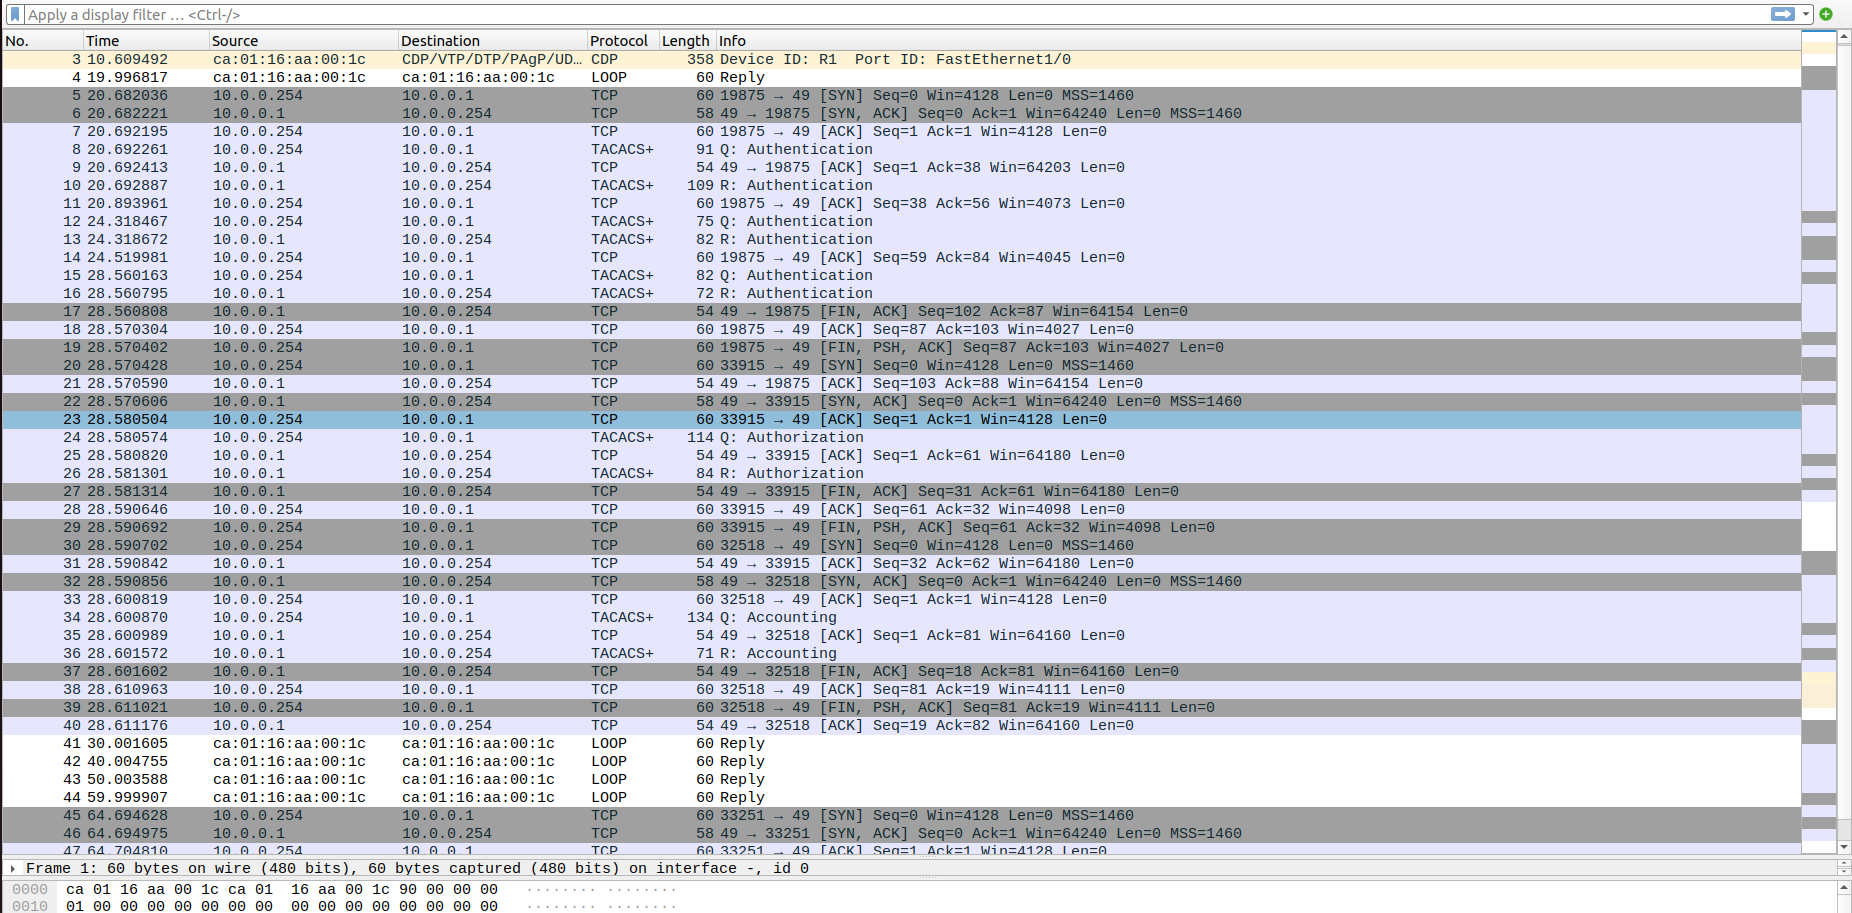
\includegraphics[width=0.9\textwidth]{../Images/TACACS+_avg_display.png}
\caption{Wireshark capture of TACACS+ authentication traffic}
\label{fig:tacacs-wireshark}
\end{figure}

Authentication packets were generated when users attempted
to log into the router. Authorization packets were exchanged
when IOS requested permission for command execution and
privilege assignment. Accounting packets were generated
when user sessions started or ended.

Because TACACS+ encrypts packet payloads, Wireshark decryption
required the shared secret configured between the router and
the TACACS+ server.

\subsubsection{Benefits of Server-Based AAA}

Compared to local AAA, server-based AAA provides centralized
management of user accounts and permissions across multiple devices.

This approach simplifies administration, improves scalability,
and enables detailed auditing of administrative activity.
TACACS+ also provides granular command authorization,
allowing different users to receive different privilege levels
and command permissions.

Overall, centralized AAA provides significantly better security,
control, and accountability than locally configured
authentication alone.

\subsection{AAA with Radius}

\subsubsection{Radius Configuration}

AAA was enabled on the router using the IOS \texttt{aaa new-model} command. A local administrative user was also configured to guarantee fallback access if the Radius server became unavailable.

\begin{verbatim}
username admin privilege 15 password 0 admin
enable password cisco
aaa new-model
\end{verbatim}

The Radius server was then configured on the router:

\begin{verbatim}
radius server Server-R
 address ipv4 10.0.0.1 auth-port 1812 acct-port 1813
 key myradiuskey
\end{verbatim}

Authentication, authorization, and accounting policies were configured as follows:

\begin{verbatim}
aaa authentication login default group radius local
aaa authorization exec default group radius local
aaa accounting exec default start-stop group radius
\end{verbatim}

Remote access through Telnet was enabled on the VTY lines:

\begin{verbatim}
line vty 0 4
 login authentication default
 transport input telnet
\end{verbatim}

On the Radius server, users were configured in the file:

\begin{verbatim}
/etc/freeradius/3.0/users
\end{verbatim}

The predefined users \texttt{bob} and \texttt{alice} were configured with password \texttt{gns3}.

The shared secret used between the Radius client and server was configured in:

\begin{verbatim}
/etc/freeradius/3.0/clients.conf
\end{verbatim}

\subsubsection{Authentication, Authorization and Accounting}

\paragraph{Authentication}

Authentication was implemented using Radius server-based login validation. When a Telnet session was initiated, R1 forwarded the supplied credentials to the Radius server for verification.

Authentication was validated by successfully logging into the router using the centralized Radius user accounts.

\begin{verbatim}
root@TelnetClient:~# telnet 222.10.10.254
Trying 222.10.10.254...
Connected to 222.10.10.254.
Escape character is '^]'.


User Access Verification

Username: bob
Password: 
Hello, bob 

R1>exit
Connection closed by foreign host.
root@TelnetClient:~# telnet 222.10.10.254
Trying 222.10.10.254...
Connected to 222.10.10.254.
Escape character is '^]'.

User Access Verification

Username: alice
Password: 
Hello, alice 

R1>exit
Connection closed by foreign host.
root@TelnetClient:~#
\end{verbatim}

\paragraph{Authorization}

Wireshark captures show that Radius exchanges mainly consist of authentication and accounting messages between R1 and the Radius server.

During user login, the router sends an \texttt{Access-Request} message containing information such as the username, NAS IP address, and authentication parameters. The Radius server then replies with either an \texttt{Access-Accept} or \texttt{Access-Reject} message, depending on the validity of the supplied credentials.

At the beginning and end of a successful administrative session, accounting messages are exchanged. The router sends \texttt{Accounting-Request} packets to report session start and stop events, while the server replies with \texttt{Accounting-Response} messages.
\begin{center}
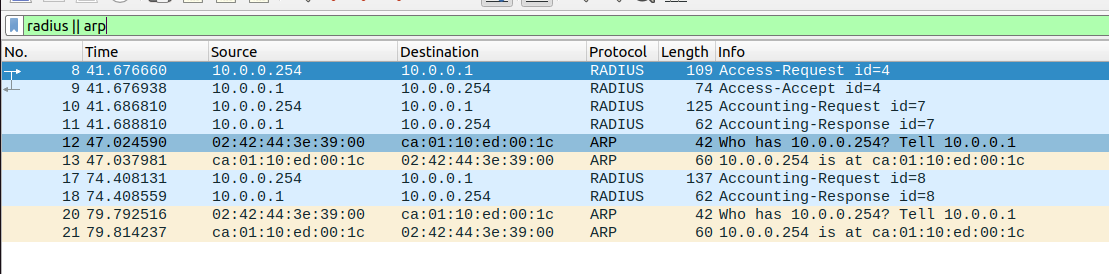
\includegraphics[width=0.75\textwidth]{../Images/radius_exec.png}
\end{center}

Unlike TACACS+, Radius generates relatively few messages during the session itself. Most Radius traffic is observed only during login and logout operations. TACACS+, on the other hand, generates additional authorization exchanges throughout the session because IOS commands can be individually authorized by the TACACS+ server.

\paragraph{Accounting}

Accounting was configured to log administrative activity on the Radius server.

Session information was stored in:

\begin{verbatim}
/var/log/freeradius/radacct/
\end{verbatim}

The generated logs contain information such as usernames, timestamps, session start and stop events, and NAS information.

\begin{verbatim}
Sat May  9 15:24:52 2026
    Acct-Session-Id = "00000001"
    User-Name = "bob"
    Acct-Authentic = RADIUS
    Acct-Status-Type = Start
    NAS-Port = 2
    NAS-Port-Id = "tty2"
    NAS-Port-Type = Virtual
    Service-Type = NAS-Prompt-User
    NAS-IP-Address = 10.0.0.254
    Acct-Delay-Time = 0
    Event-Timestamp = "May  9 2026 15:24:52 UTC"
    Tmp-String-9 = "ai:"
    Acct-Unique-Session-Id = "5f17e8201ba1e8d959a54331f562dbd0"
    Timestamp = 1778340292

Sat May  9 15:25:00 2026
    Acct-Session-Id = "00000001"
    User-Name = "bob"
    Acct-Authentic = RADIUS
    Acct-Terminate-Cause = User-Request
    Acct-Session-Time = 8
    Acct-Status-Type = Stop
    NAS-Port = 2
    NAS-Port-Id = "tty2"
    NAS-Port-Type = Virtual
    Service-Type = NAS-Prompt-User
    NAS-IP-Address = 10.0.0.254
    Acct-Delay-Time = 0
    Event-Timestamp = "May  9 2026 15:25:00 UTC"
    Tmp-String-9 = "ai:"
    Acct-Unique-Session-Id = "5f17e8201ba1e8d959a54331f562dbd0"
    Timestamp = 1778340300

Sat May  9 15:25:07 2026
    Acct-Session-Id = "00000002"
    User-Name = "alice"
    Acct-Authentic = RADIUS
    Acct-Status-Type = Start
    NAS-Port = 2
    NAS-Port-Id = "tty2"
    NAS-Port-Type = Virtual
    Service-Type = NAS-Prompt-User
    NAS-IP-Address = 10.0.0.254
    Acct-Delay-Time = 0
    Event-Timestamp = "May  9 2026 15:25:07 UTC"
    Tmp-String-9 = "ai:"
    Acct-Unique-Session-Id = "683333e47c0de024a04e881f984026f2"
    Timestamp = 1778340307
\end{verbatim}

\subsubsection{Comparison Between TACACS+ and Radius}

Although both TACACS+ and Radius provide centralized AAA services, important differences exist between the two protocols.

TACACS+ uses TCP port 49, while Radius uses UDP ports 1812 and 1813. TACACS+ encrypts the entire packet payload, whereas Radius encrypts only the password field.

Another important difference is that TACACS+ separates authentication, authorization, and accounting into independent processes and supports per-command authorization for IOS devices. Radius combines authentication and authorization and does not support granular IOS command authorization.

Radius is widely used for network access authentication, while TACACS+ is more commonly used for administrative access control in Cisco environments.

Overall, TACACS+ provides more granular administrative control, while Radius offers broader interoperability and simpler deployment.

\newpage

\subsection{802.1X Authentication}

IEEE 802.1X authentication was implemented using
a Cisco IOSvL2 switch as the authenticator,
a Linux host running \texttt{wpa\_supplicant}
as the supplicant, and a FreeRADIUS server
as the authentication server.

The switch ports were configured for 802.1X
port-based authentication using RADIUS.

\begin{configbox}
aaa new-model
aaa authentication dot1x default group radius

radius server AAAServer
 address ipv4 10.1.1.50 auth-port 1812 acct-port 1813
 key gns3

dot1x system-auth-control
\end{configbox}

The supplicant configuration used PEAP
with MSCHAPv2 authentication:

\begin{configbox}
network={
    key_mgmt=IEEE8021X
    eap=PEAP
    identity="bob"
    password="gns3"
    phase2="auth=MSCHAPV2"
}
\end{configbox}

Authentication was initiated using:

\begin{configbox}
wpa_supplicant -Dwired -ieth0 -c/usr/wpa.conf
\end{configbox}

Successful authentication was confirmed on the
Cisco switch through the authenticated session table.

\begin{figure}[H]
\centering
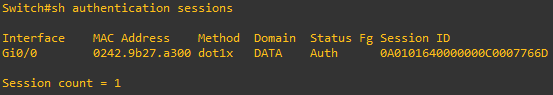
\includegraphics[width=0.85\textwidth]{../Images/show_authentication_sessions.png}
\caption{Authenticated 802.1X session on the Cisco switch}
\label{fig:8021x-auth}
\end{figure}

\subsubsection{Wireshark Analysis of EAP-PEAP Authentication}

Wireshark was used to capture and analyze the
EAP-PEAP authentication exchange between the
supplicant and the switch.

The captures show the complete IEEE 802.1X
authentication process, including:

\begin{itemize}
\item EAPOL-Start
\item EAP Request Identity
\item EAP Response Identity
\item Protected EAP (PEAP)
\item TLS handshake messages
\item EAP Success
\end{itemize}

\begin{figure}[H]
\centering
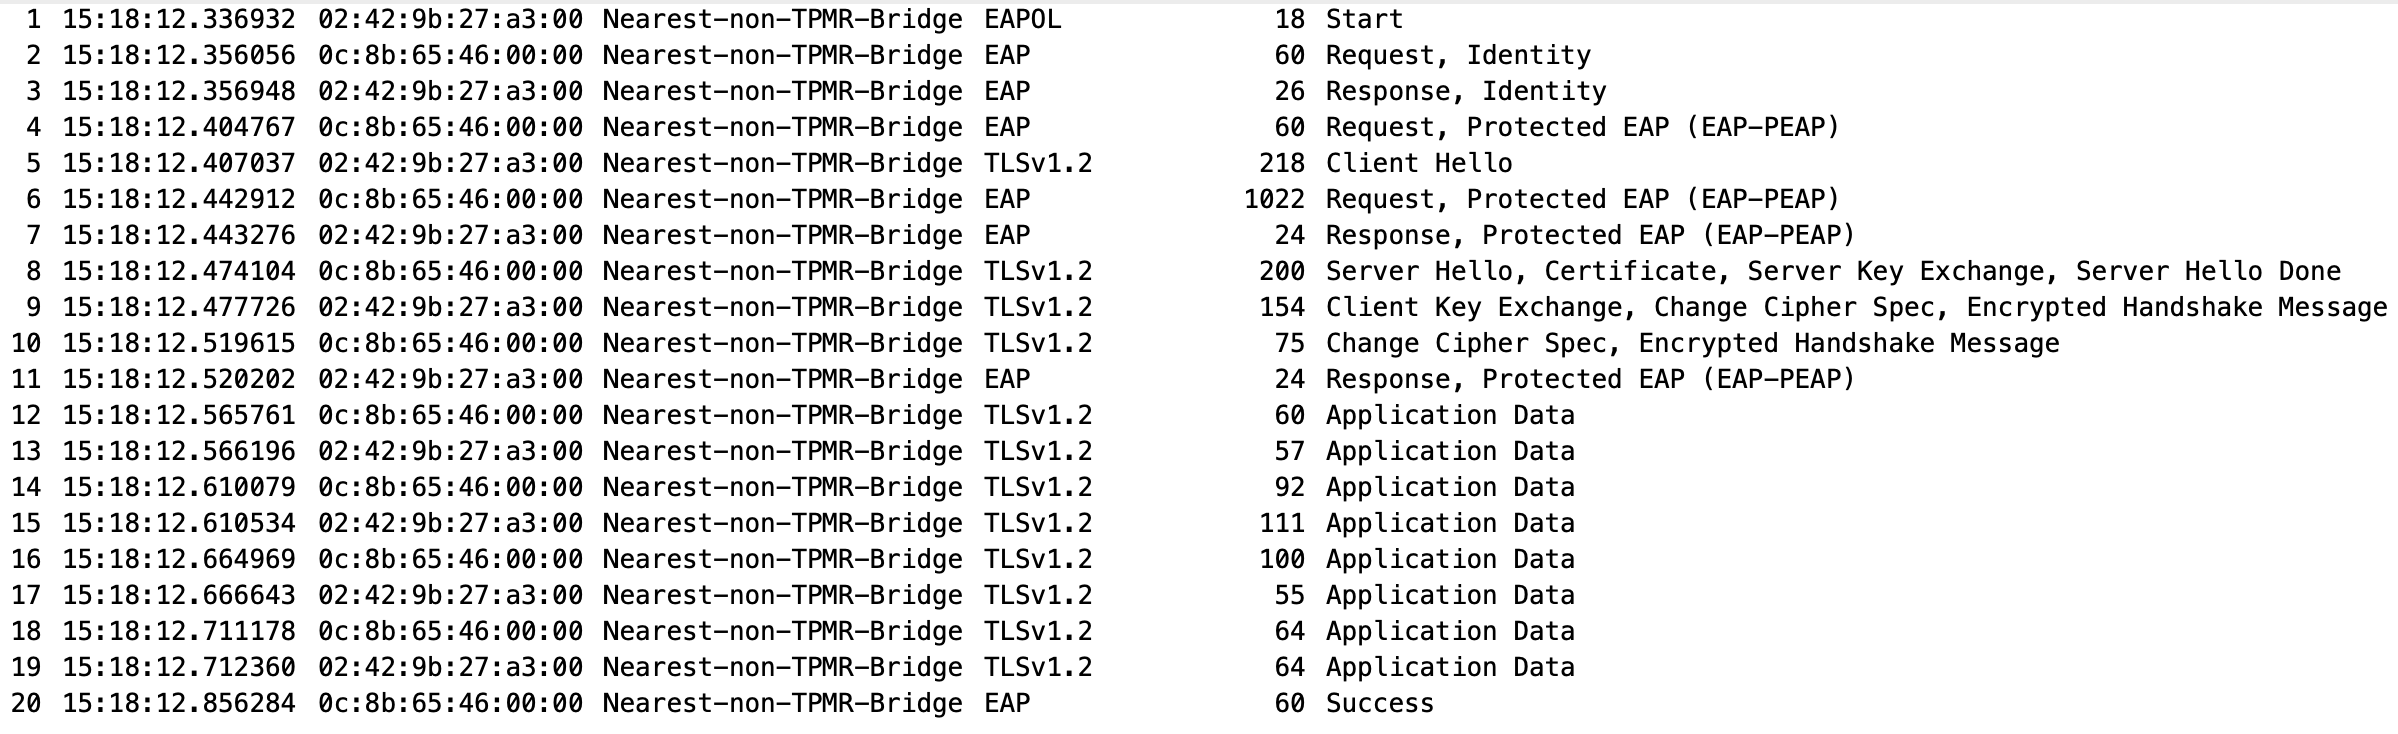
\includegraphics[width=\textwidth]{../Images/eap_peap_capture.png}
\caption{Wireshark capture of the EAP-PEAP authentication process}
\label{fig:eap-peap-capture}
\end{figure}

The authentication process starts when the
supplicant sends an EAPOL-Start frame after
connecting to the switch port.

The switch, acting as the authenticator,
responds with an EAP Request Identity message.
The supplicant then replies with an EAP Response
Identity containing the username used for authentication.

\begin{figure}[H]
\centering
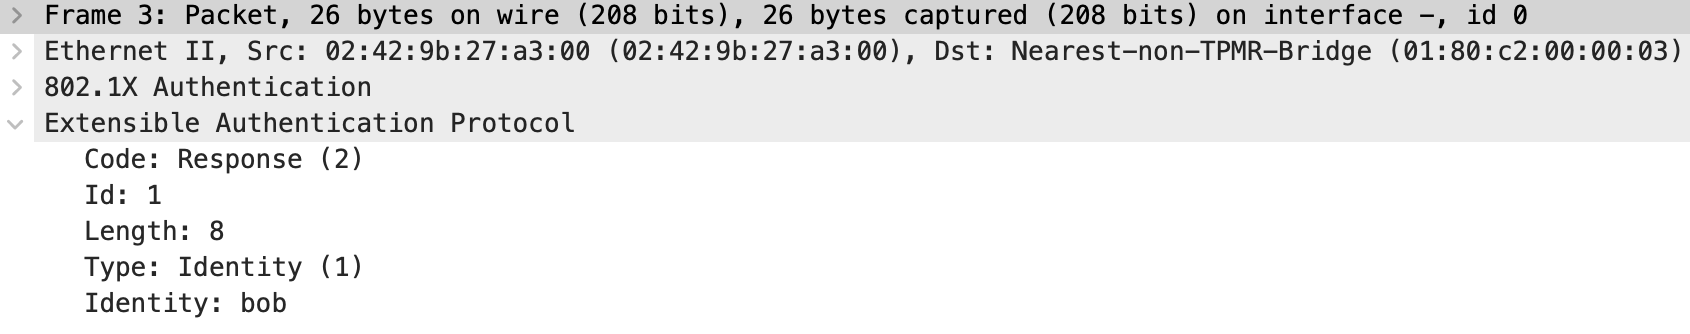
\includegraphics[width=0.8\textwidth]{../Images/response_identity_packet.png}
\caption{EAP Response Identity packet containing the username used during authentication}
\label{fig:eap-identity}
\end{figure}

The EAP Response Identity packet contains the
username provided by the supplicant during
the authentication exchange.

In this setup, the supplicant identified itself
using the username \texttt{bob}, which was later
validated by the FreeRADIUS server through
PEAP/MSCHAPv2 authentication.

The switch forwards the authentication information
to the FreeRADIUS server using the RADIUS protocol.

PEAP negotiation is then initiated in order to
establish a TLS tunnel between the supplicant
and the authentication server.
The Wireshark captures show TLS handshake
messages, including Client Hello and Change Cipher Spec.

After the TLS tunnel is established,
MSCHAPv2 authentication takes place inside
the encrypted channel.

Finally, the authentication process completes
successfully with the EAP Success message,
allowing the switch to authorize the port
for normal network access.

\subsubsection{Security Considerations}

IEEE 802.1X authentication can mitigate several
network attacks studied in Lab 1.1.

By requiring authentication before granting
access to switch ports, unauthorized devices
cannot easily connect to the network.

This mechanism helps mitigate:

\begin{itemize}
\item Unauthorized network access
\item Rogue devices connected to switch ports
\item Basic MAC spoofing attempts
\item Passive credential sniffing attacks
\end{itemize}

The use of PEAP additionally protects
authentication credentials by establishing
an encrypted TLS tunnel between the supplicant
and the authentication server.

However, IEEE 802.1X does not directly mitigate
Denial of Service attacks such as ICMP flood
or TCP SYN flood attacks studied previously.

\subsubsection{Comparison Between AI Explanation and Observed Traffic}

An AI tool was used to explain the EAP-PEAP
authentication process implemented in the lab setup.

The AI explanation correctly identified the
three main entities involved in IEEE 802.1X authentication:

\begin{itemize}
\item Supplicant
\item Authenticator
\item Authentication Server
\end{itemize}

The supplicant corresponds to the Linux host
running \texttt{wpa\_supplicant}, which initiates
the authentication process and provides user credentials.

The authenticator corresponds to the Cisco switch,
which controls access to the network port and forwards
EAP messages between the supplicant and the RADIUS server.

The authentication server corresponds to the
FreeRADIUS server, which validates credentials
and decides whether authentication succeeds or fails.

The Wireshark captures confirmed the behavior
described by the AI explanation.
Observed traffic included EAPOL-Start,
Identity exchange messages, PEAP negotiation,
TLS handshake packets, and the final EAP Success message.

One important observation is that the switch
does not authenticate the user directly.
Instead, the switch acts only as an intermediary
between the supplicant and the FreeRADIUS server.
The actual authentication decision is performed
exclusively by the RADIUS server.

Overall, the AI explanation was consistent
with the observed protocol behavior and packet captures.
\newpage

\section{Conclusion}

\newpage

\section{Appendix}

\end{document}